\section{Modification}

The Python adaptation is a close adaptation of the original MATLAB scripts provided by the authors. However, on simulating their performance on the three tasks, we observed that while, for the first two tasks, the models performed as described in \textcite{pyle2019}, the performance of the SUPERTREX algorithm on Task 3 was not consistent, and was dependent on the seed used for the random number generator. On inspecting further, we notice that this was, in some cases, due to the uncontrolled exponential increase in the readout weights.\\

To look into the robustness of the implementations further, we test the performance of the RMHL and SUPERTREX algorithms on Task 2 with certain modifications to the task parameters, specifically, the number of arm segments and the length of the arm segments. It would be expected for the behaviour to be comparable with the performance on the original task performance, or undergo a gradual decline. We test Task 2 on the arm parameters, which were used in Task 3, i.e. by increasing the number of arm segments from two to three and changing the length of each arm segment. We observe that RMHL performance is comparable to the original Task 2, wherein the time series is generated during the training phase, but is not maintained beyond (Original scripts: $0.846\pm0.299$, Python adaptation: $0.738\pm0.256$; n=11).  On the other hand, simulations of the SUPERTREX model, with 2 out of 11 seeds, were able to produce the target output satisfactorily (Original scripts: $0.016\pm0.007$, Python adaptation: $0.009\pm0.003$; n=2) (Figure~\ref{Fig:Comparison_Task2_Seg3}). However, in simulations with 9 out of 11 seeds, the weights increase exponentially, rendering the simulation unable to progress in a meaningful manner (Table~\ref{Table:deviation_tasks},~\ref{Table:deviation_prop_tasks}). \\
    


\begin{figure}


    \centering
    
    \hspace{2em}
    \textbf{MATLAB}\hspace{10em}
    \textbf{Python with modification}
    
    \hspace{-2em}
    
\includegraphics[trim=3cm 4cm 3cm 4cm, clip=true, height=.25\linewidth]{Figures/Fig_T5/MATLAB/ST_T2_Seg3_Var_Trajectory.eps}
    \hspace{4em}
    
\includegraphics[trim=6.5cm 4.5cm 6cm 4.5cm, clip=true,  height=.25\linewidth]{Figures/Fig_T5/ImprovP/ST_T2_Seg3_Var_Trajectory.eps} \\
    

    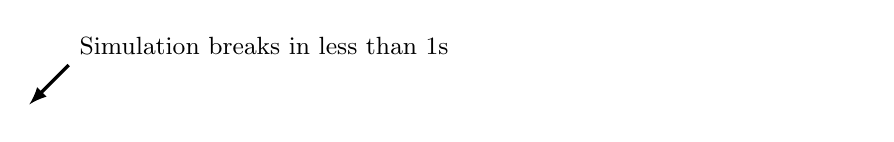
\begin{tikzpicture}  \node (image) at (0,0) {
    };
    \draw[latex-, very thick,black] (-10.5,0)  -- (-10,0.5)
        node[anchor=south west,black,fill=white]{\small Simulation breaks in less than 1s};
        
    \end{tikzpicture}
    \textbf{\rotatebox{90}{$\theta_1$}}\begin{subfigure}{\textwidth}
        \centering

        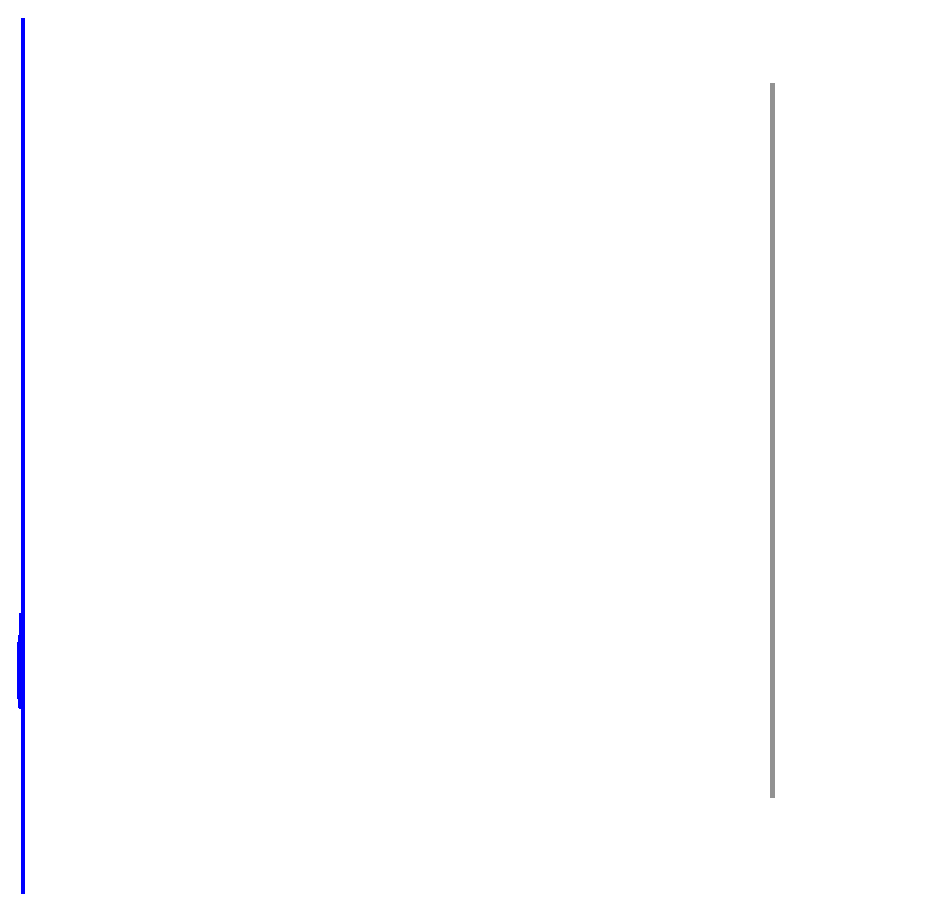
\includegraphics[trim=0cm 0cm 0cm 0cm,clip=true,height=0.1\linewidth,width=.45\linewidth]{Figures/Fig_T5/MATLAB/ST_T2_Seg3_Var_Theta0.eps}
        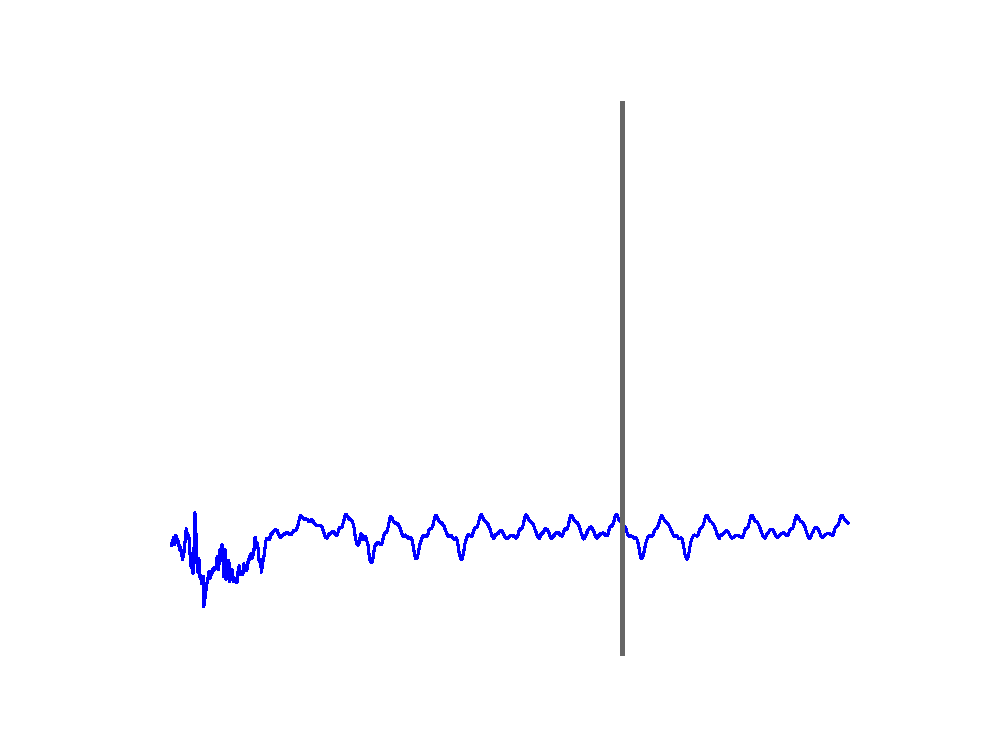
\includegraphics[trim=2cm 1cm 2cm 1cm,clip=true,height=0.1\linewidth,width=.45\linewidth]{Figures/Fig_T5/ImprovP/ST_T2_Seg3_Var_Theta0.eps}

    \end{subfigure}
    
        
        
    \textbf{\rotatebox{90}{$\theta_2$}}\begin{subfigure}{\textwidth}
        \centering
        
        \includegraphics[trim=0cm 0cm 0cm 0cm,clip=true,height=0.1\linewidth,width=.45\linewidth]{Figures/Fig_T5/MATLAB/ST_T2_Seg3_Var_Theta1.eps}
        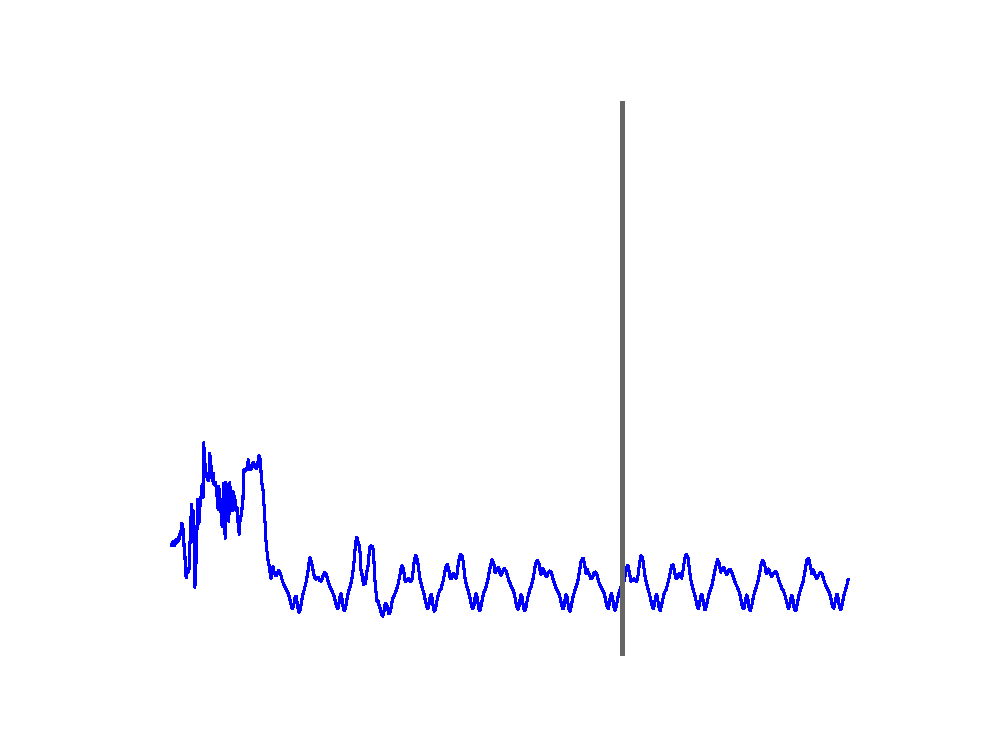
\includegraphics[trim=2cm 1cm 2cm 1cm,clip=true,height=0.1\linewidth,width=.45\linewidth]{Figures/Fig_T5/ImprovP/ST_T2_Seg3_Var_Theta1.eps}   

    \end{subfigure}
    
    
    \textbf{\rotatebox{90}{$\theta_3$}}\begin{subfigure}{\textwidth}
        \centering
        
        
\includegraphics[trim=0cm 0cm 0cm 0cm,clip=true,height=0.1\linewidth,width=.45\linewidth]{Figures/Fig_T5/MATLAB/ST_T2_Seg3_Var_Theta2.eps}
        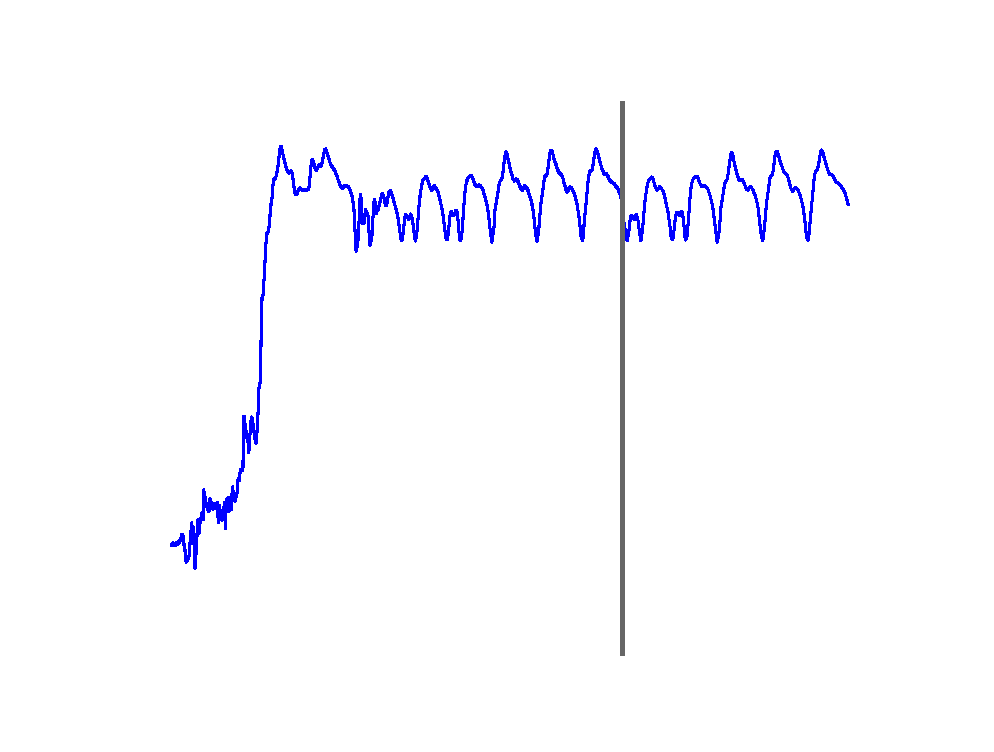
\includegraphics[trim=2cm 1cm 2cm 1cm,clip=true,height=0.1\linewidth,width=.45\linewidth]{Figures/Fig_T5/ImprovP/ST_T2_Seg3_Var_Theta2.eps}  
    
    \end{subfigure}
    
    \vspace{4em}
    
    \textbf{\rotatebox{90}{$||W||$}}\begin{subfigure}{\textwidth}
        \centering
        
        \hspace{.5em}
        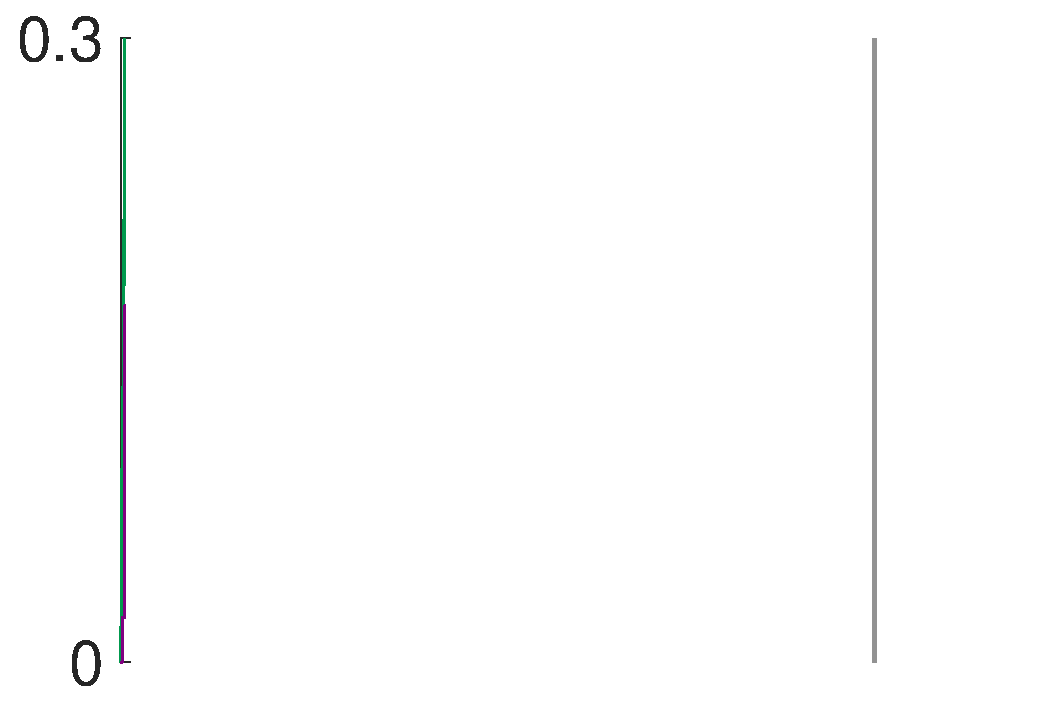
\includegraphics[trim=0cm 0cm 0cm 0cm,clip=true,height=0.15\linewidth,width=.45\linewidth]{Figures/Fig_T5/MATLAB/ST_T2_Seg3_Var_W_norm.eps}
        \hspace{0em}
        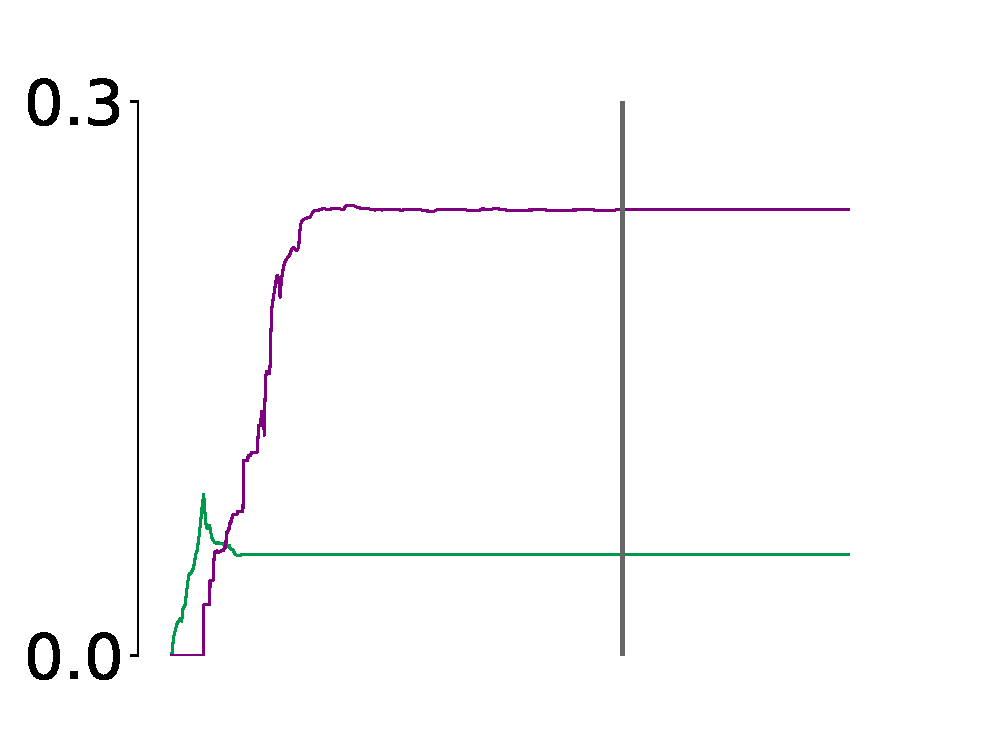
\includegraphics[trim=0cm 0cm 0cm 0cm,clip=true,height=0.15\linewidth,width=.45\linewidth]{Figures/Fig_T5/ImprovP/ST_T2_Seg3_Var_W_norm.eps}
    
    \end{subfigure}
    
    
    \vspace{4em}
    
    \textbf{\rotatebox{90}{MSE}}\begin{subfigure}{\textwidth}
        \centering
        
        \hspace{-.5em}
    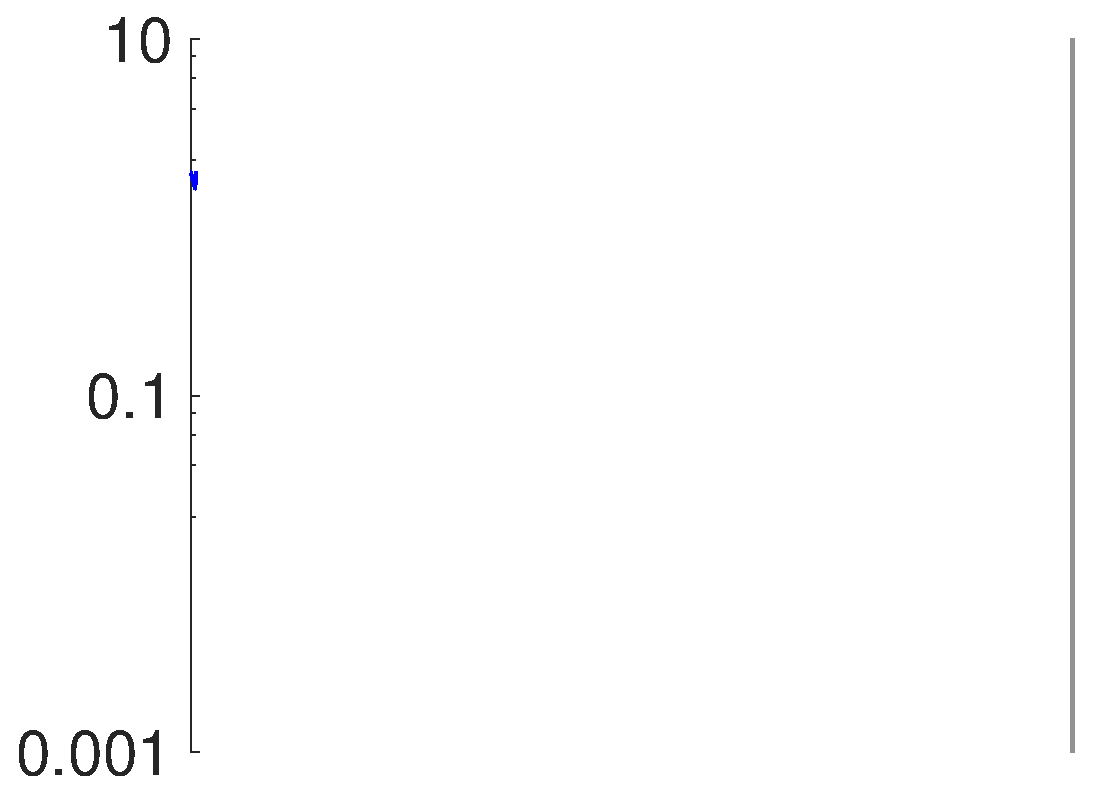
\includegraphics[trim=0cm 0cm 0cm 0cm,clip=true,height=0.15\linewidth,width=.4\linewidth]{Figures/Fig_T5/MATLAB/ST_T2_Seg3_Var_MSE.eps}
        \hspace{1.5em}
        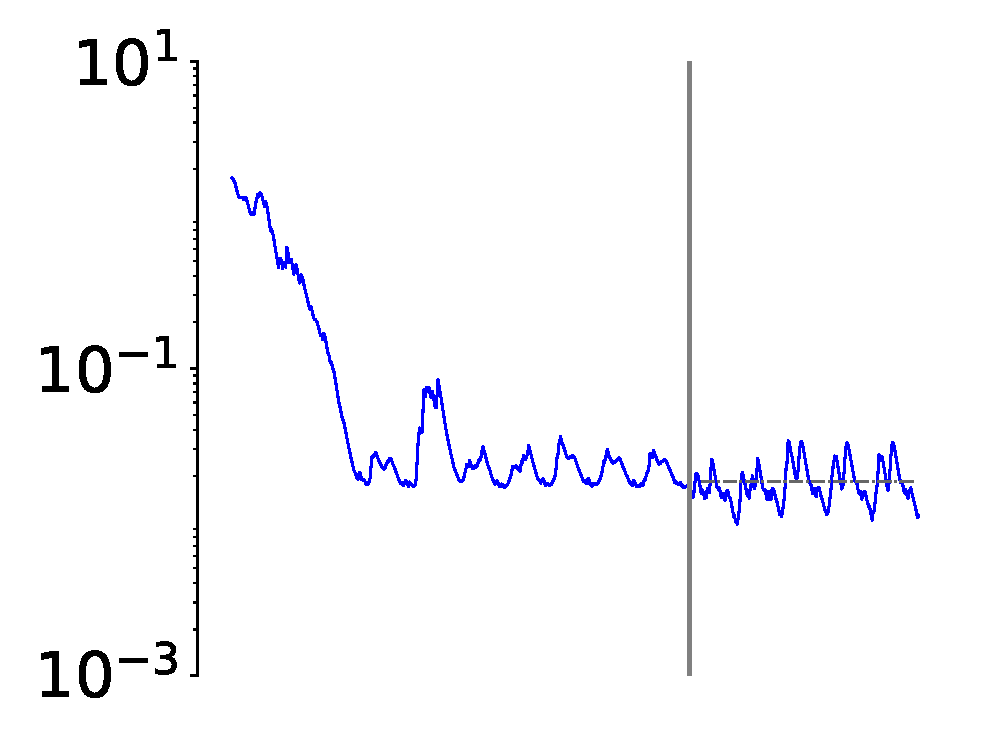
\includegraphics[trim=0cm 0cm 0cm 0cm,clip=true,clip=true,height=0.15\linewidth,width=.45\linewidth]{Figures/Fig_T5/ImprovP/ST_T2_Seg3_Var_MSE.eps}
    
    \end{subfigure}
        
    
        
        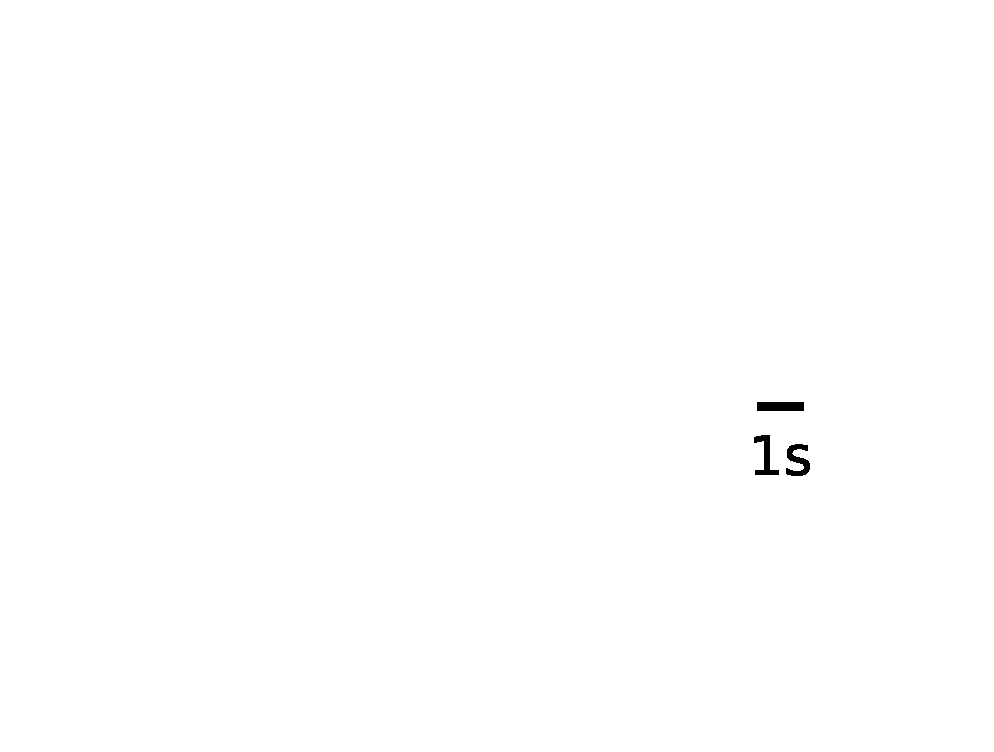
\includegraphics[trim=2cm 6cm 2cm 6cm, clip=true,height=0.05\linewidth,width=.4\linewidth]{Figures/Fig_T1/Python/ST_T1_Scale.eps}
        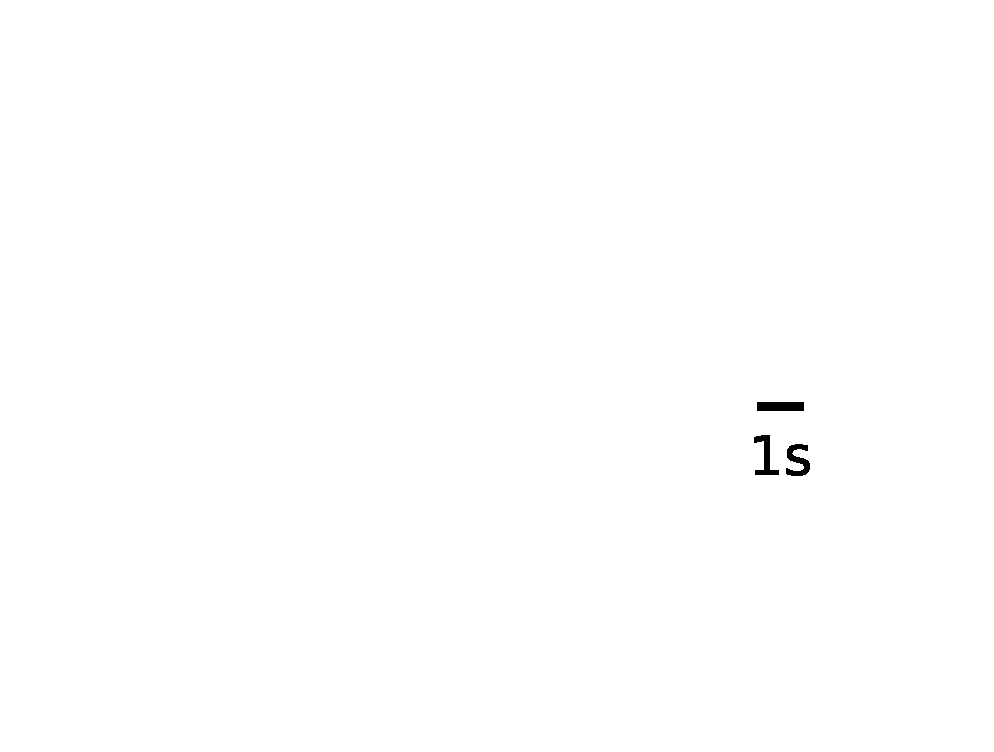
\includegraphics[trim=2cm 4cm 2cm 6cm, clip=true,height=0.05\linewidth,width=.45\linewidth]{Figures/Fig_T1/Python/ST_T1_Scale.eps}



\caption{Robustness of the SUPERTREX model on a Task 2 variant. The performance of the original scripts (left column) and modified Python re-implementation (right column) is tested for the SUPERTREX learning algorithm on a variant of Task 2 with increased number of arm segments (lengths: 1.8, 1.2, 0.6). The top panel shows the target trajectory (red) with the trajectory generated by the algorithm (blue) throughout the test phase. The next three rows show the time-series (blue) generated by the model (joint angles ($\theta_i$), in this case). The fourth row shows the progression of the norm of the weight matrix ($W_1$ in purple; $W_2$, in green). The bottom row shows the distance from target metric (blue) over the simulation, using the log scale for the y axis. The horizontal grey line, in the test phase, indicates the deviation metric. The grey vertical line marks the separation of the training and testing phase. Using the MATLAB scripts, the readout weights increase uncontrollably rendering the model unable to learn. The Python re-implementation, using a compensation factor to harness the weight update, is able to learn and converge to produce the target time-series.}
\label{Fig:Comparison_Task2_Seg3}

\end{figure}



In order to improve the model performance, make the model more scalable in terms of task parameters, and also more robust (as seen in Task 3, with respect to reproducibility with different random seeds), we introduce two minor alterations.

\begin{enumerate}
    \item We introduce a compensation factor to the update of the readout weights in the exploratory pathway, inversely proportional to the number of segments. Specifically, when the number of segments is greater than two, we multiply the weight update by $0.1/n\_segs$ for Task 2 and by $0.5/n\_segs$ for Task 3.
    \item The SUPERTREX model transfers the information from the exploratory pathway to the mastery pathway, only if the error is consistently below a certain threshold. In the original scripts, this threshold is set at 1.5e-3 for Task 1 and Task 2, while at 1.5e-2 for Task 3. We change the transfer threshold for Task 2 from 1.5e-3 to 1.5e-2. 
\end{enumerate}

These slight modifications address the shortcomings we encountered earlier with the performance of SUPERTREX in Task 2 and 3. Alteration \#1, by including a compensation factor for the change in number of arm segments, prevents the weights from increasing exponentially, and lets the simulation proceed in a meaningful manner. Alteration \#2, by increasing the error threshold governing the transfer of information to the mastery pathway, makes the model more tolerant of fluctuations, while continuing to explore and learn a good solution. Although this does not lead to a critical change for Task 1 (Original scripts: $0.006\pm0.003$, n=11; Modified Python re-implementation: $0.004\pm0.003$, n=11) and Task 2 (Original scripts: $0.011\pm0.003$, n=11; Modified Python re-implementation: $0.010\pm0.004$, n=11), this alteration improves the performance of SUPERTREX on Task 3 (Original scripts: $0.881\pm0.224$, n=11; Modified Python re-implemen\-tation: $0.140\pm0.071$, n=11). Simulations with 10 out of 11 seeds had satisfactory performance (Deviation $< 0.5$), compared to 6 out of 11 simulations for the original scripts. Further, it unlocks the potential for the model to be more scalable. We find that with these alterations, on merely increasing the number of time-steps per training cycle and with no further fine tuning of hyper-parameters, the model is able to proceed without an exponential increase in weights over a wider range of task parameters. For instance, on adding surplus segments with length 0.1 each, the model is able to perform in a satisfactory manner, for most cases, with up to 50 arm segments (Table~\ref{Table:deviation_scalability}, Figure~\ref{Fig:Scalability_Task2}). Better accuracy can be achieved by further fine tuning of the hyper-parameters.




\begin{table}[h!]
\begin{center}
 \begin{tabular}{||c | c | c c c ||} 
 \hline
   \multicolumn{2}{||c|}{Task 2 variant} & \multicolumn{3}{c||}{Deviation metric} \\ [0.5ex] 
\hline
No. of segments & Time steps & Mean & Median & Standard Deviation \\ [0.5ex] 
 \hline\hline
 3 & 10000 & 0.057 &	0.032 &	0.069 \\ 
 \hline
 4 & 10000 & 0.242 &	0.221 &	0.136 \\ 
 \hline
 5 & 10000 & 0.141 &	0.080 &	0.147 \\ 
 \hline
 6 & 10000 & 0.181 &	0.160 &	0.133 \\ 
 \hline
 7 & 10000 & 0.173 &	0.129 &	0.130 \\ 
 \hline
 8 & 10000 & 0.253 &	0.230 &	0.137 \\ 
 \hline
 9 & 10000 & 0.331 &	0.297 &	0.168 \\ 
 \hline
 10 & 10000 & 0.417 &	0.409 &	0.151 \\ 
 \hline
 15 & 10000 & 0.538 &	0.512 &	0.179 \\ 
 \hline 
 20 & 15000 & 0.366 &	0.324 &	0.188 \\ 
 \hline
 30 & 20000 & 0.549 &	0.489 &	0.236 \\ 
 \hline
 40 & 20000 & 0.372 &	0.313 &	0.228 \\ 
 \hline
 50 & 30000 & 0.375 &	0.283 &	0.281 \\ [1ex] 
 \hline
\end{tabular}
\end{center}
 \caption{Deviation metric showing the performance of the modified Python implementation on increasing number of segments for Task 2. Each variant is simulated with the default seed (5489) and ten additional seeds. The mean, median and standard deviation of the deviation metric over these eleven simulations are tabulated here.}
 \label{Table:deviation_scalability}
\end{table}




\begin{figure}

        \textbf{\rotatebox[origin=c]{90}{\hspace{-7.5em} MSE \hspace{2.5em} y(t) \hspace{1.5em} x(t)}}
        \begin{subfigure}{\textwidth}
            \centering
    
            \textbf{5 segments}\hspace{12em}\textbf{6 segments}
            
            
\includegraphics[trim=5cm 4cm 5cm 4cm, clip=true,height=0.15\linewidth]{Figures/Fig_T6/ImprovP/ST_T2_Seg5_Var_Trajectory.eps}
            \hspace{9em}
            \includegraphics[trim=5cm 4cm 5cm 4cm, clip=true,height=0.15\linewidth]{Figures/Fig_T6/ImprovP/ST_T2_Seg6_Var_Trajectory.eps}
            %trim=1cm 0cm 0cm 0cm, clip=true,
            
            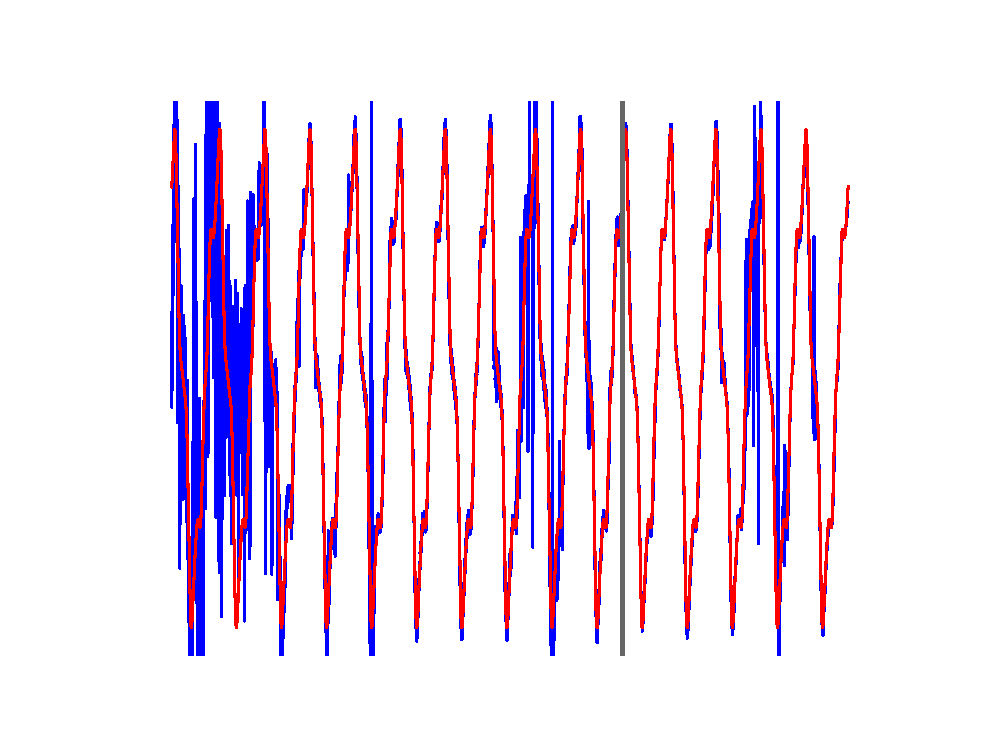
\includegraphics[trim=2cm 1cm 2cm 1cm, clip=true,height=0.1\linewidth,width=.45\linewidth]{Figures/Fig_T6/ImprovP/ST_T2_Seg5_Var_CoordinateX.eps} 
            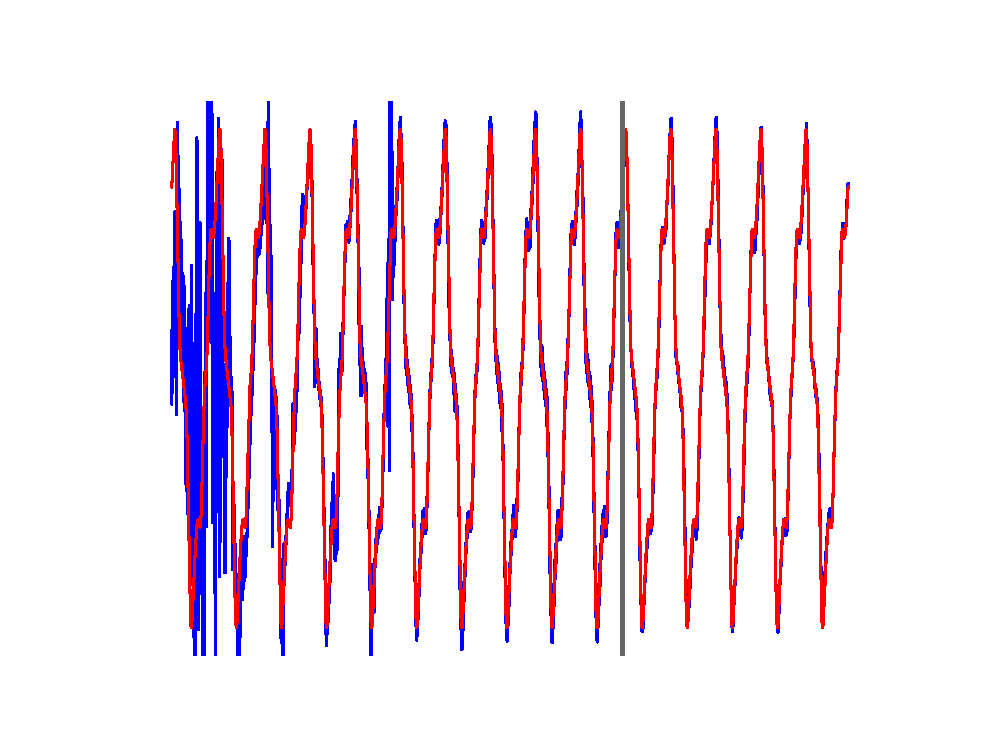
\includegraphics[trim=2cm 1cm 2cm 1cm, clip=true,height=0.1\linewidth,width=.45\linewidth]{Figures/Fig_T6/ImprovP/ST_T2_Seg6_Var_CoordinateX.eps}       

            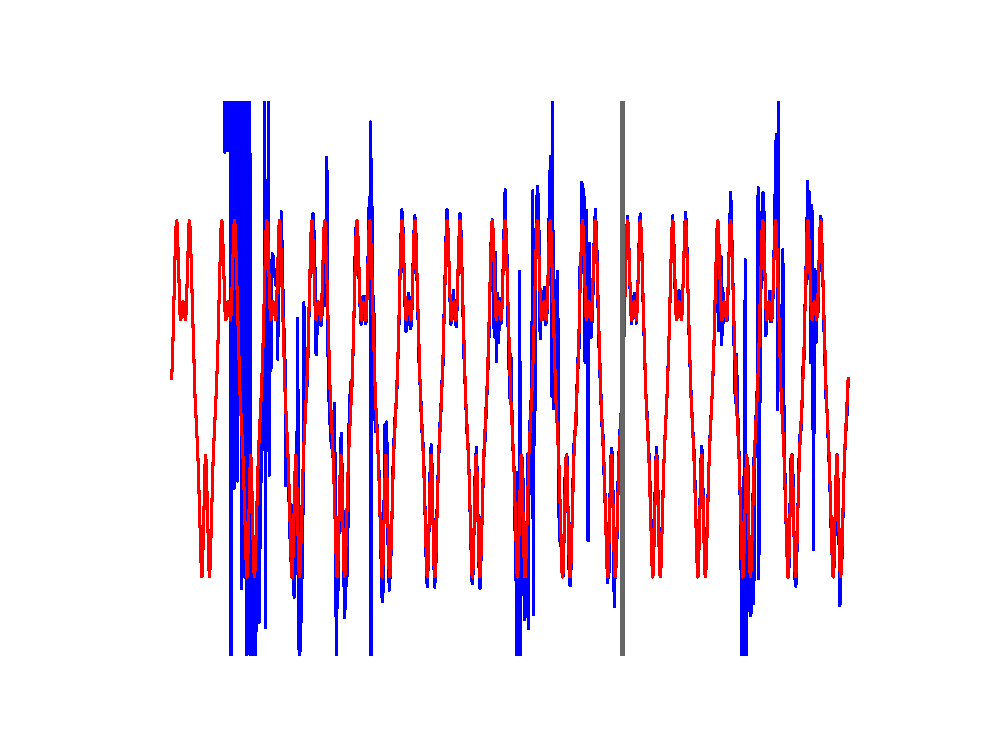
\includegraphics[trim=2cm 1cm 2cm 1cm, clip=true,height=0.1\linewidth,width=.45\linewidth]{Figures/Fig_T6/ImprovP/ST_T2_Seg5_Var_CoordinateY.eps}    
            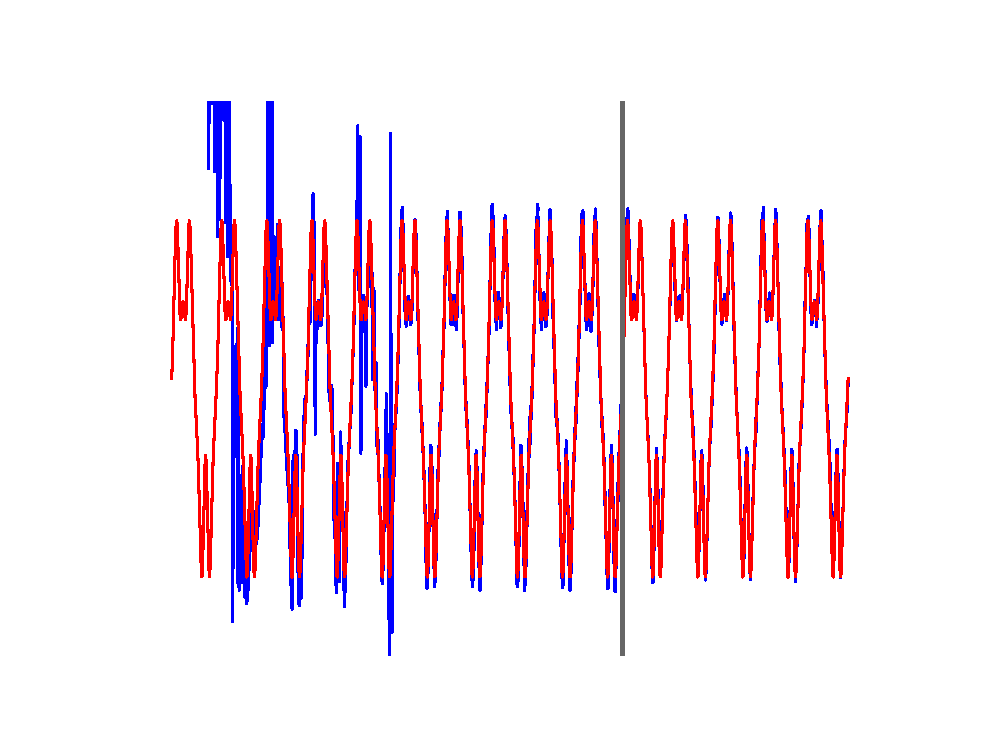
\includegraphics[trim=2cm 1cm 2cm 1cm, clip=true,height=0.1\linewidth,width=.45\linewidth]{Figures/Fig_T6/ImprovP/ST_T2_Seg6_Var_CoordinateY.eps} 

            \hspace{-1em}
            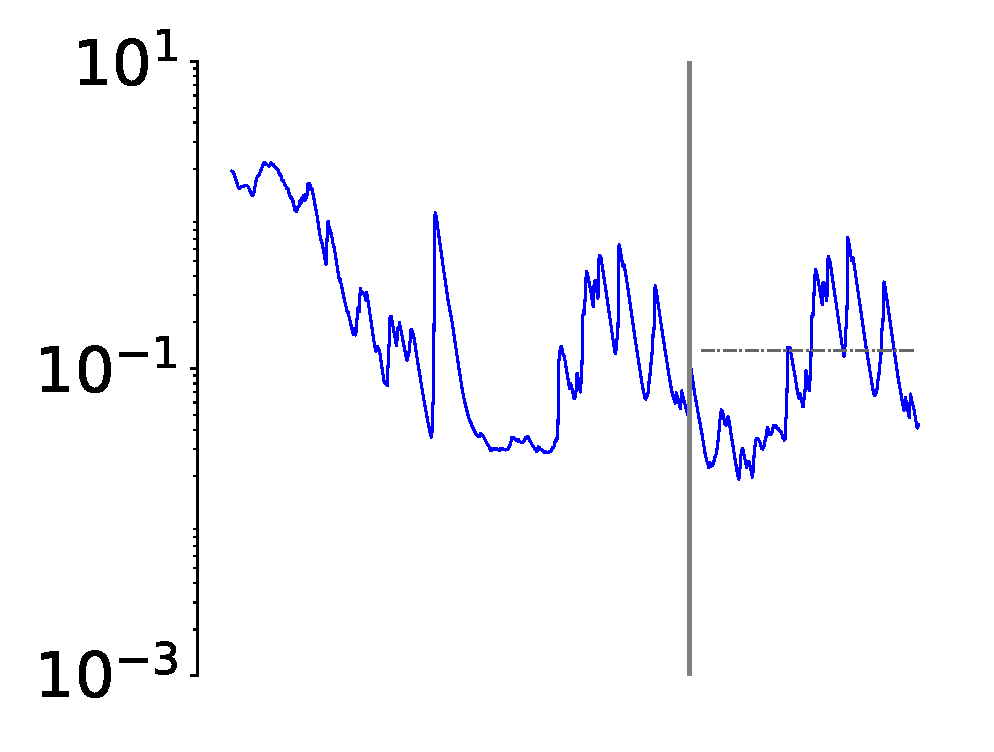
\includegraphics[height=0.15\linewidth,width=.45\linewidth]{Figures/Fig_T6/ImprovP/ST_T2_Seg5_Var_MSE.eps}
            \hspace{0em}
            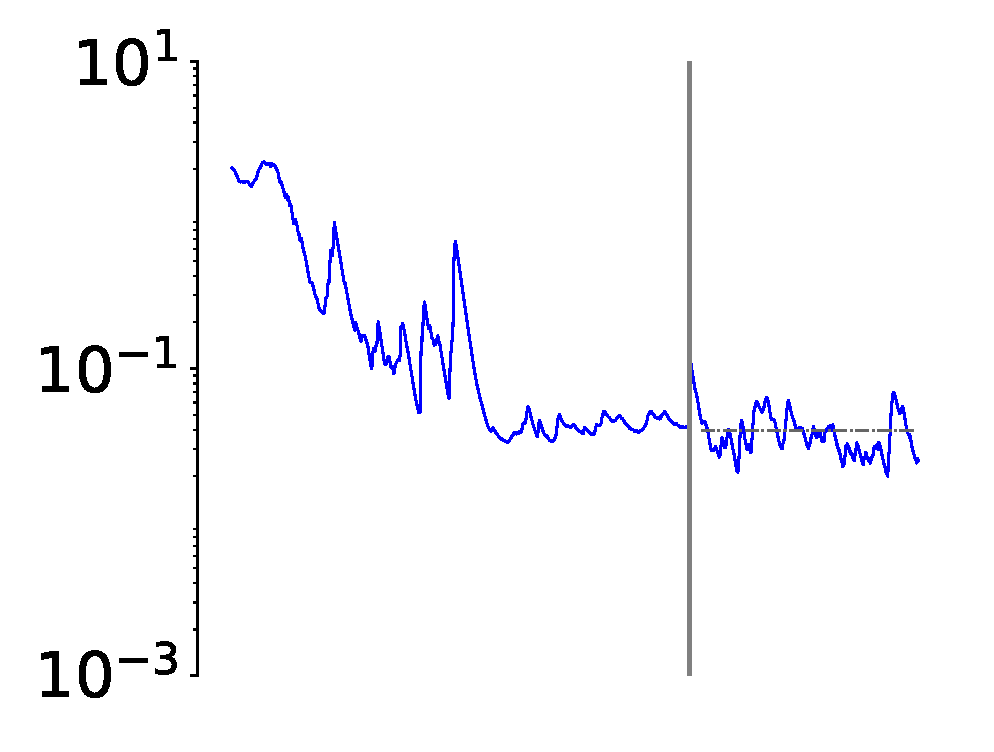
\includegraphics[height=0.15\linewidth,width=.45\linewidth]{Figures/Fig_T6/ImprovP/ST_T2_Seg6_Var_MSE.eps}

        \end{subfigure}
        
        \textbf{\rotatebox[origin=c]{90}{\hspace{-7.5em} MSE \hspace{2.5em} y(t) \hspace{1.5em} x(t)}}
        \begin{subfigure}{\textwidth}
            \centering
    
            \textbf{7 segments}\hspace{12em}\textbf{8 segments}
            
            
\includegraphics[trim=5cm 4cm 5cm 4cm, clip=true,height=0.15\linewidth]{Figures/Fig_T6/ImprovP/ST_T2_Seg7_Var_Trajectory.eps}
            \hspace{9em}
            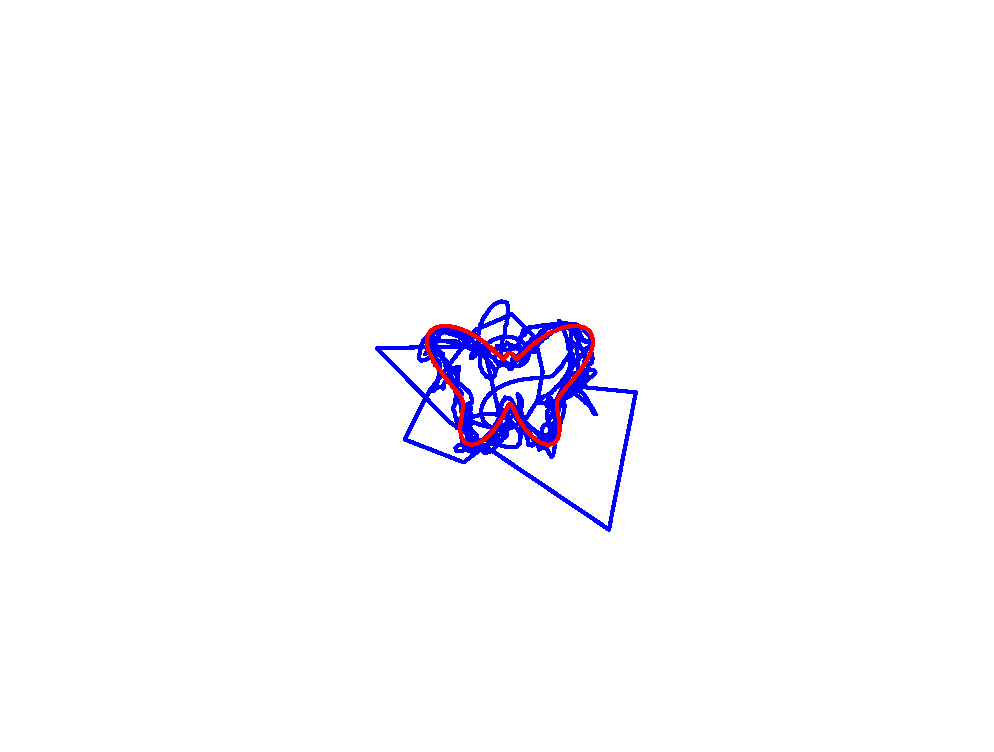
\includegraphics[trim=5cm 4cm 5cm 4cm, clip=true,height=0.15\linewidth]{Figures/Fig_T6/ImprovP/ST_T2_Seg8_Var_Trajectory.eps}
            %trim=1cm 0cm 0cm 0cm, clip=true,
            
            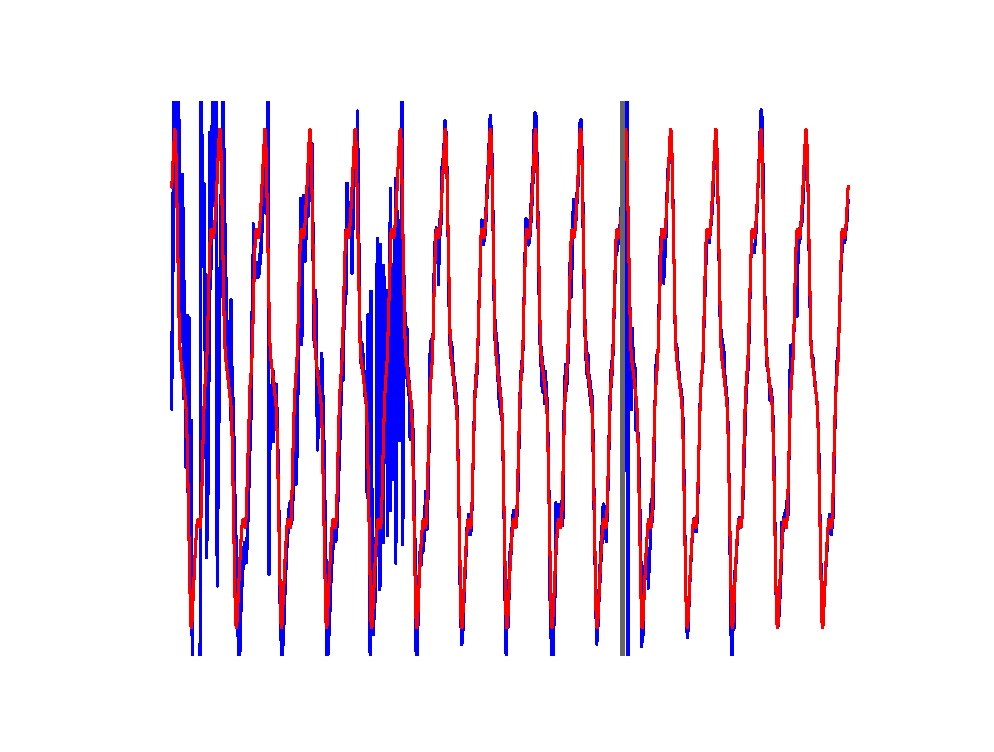
\includegraphics[trim=2cm 1cm 2cm 1cm, clip=true,height=0.1\linewidth,width=.45\linewidth]{Figures/Fig_T6/ImprovP/ST_T2_Seg7_Var_CoordinateX.eps} 
            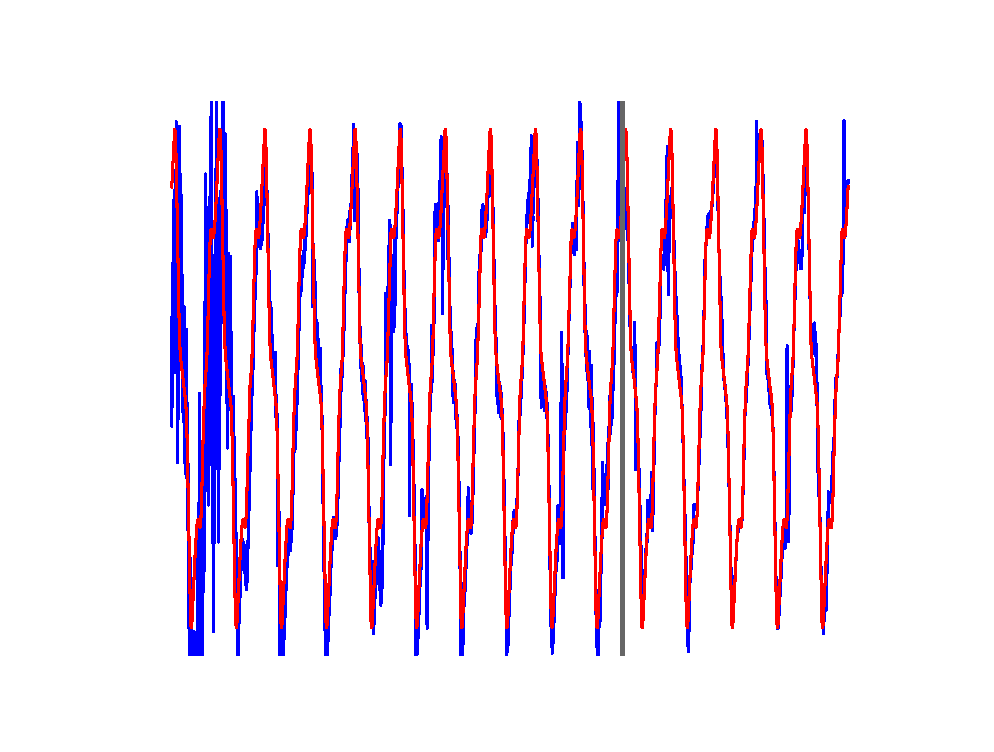
\includegraphics[trim=2cm 1cm 2cm 1cm, clip=true,height=0.1\linewidth,width=.45\linewidth]{Figures/Fig_T6/ImprovP/ST_T2_Seg8_Var_CoordinateX.eps}       

            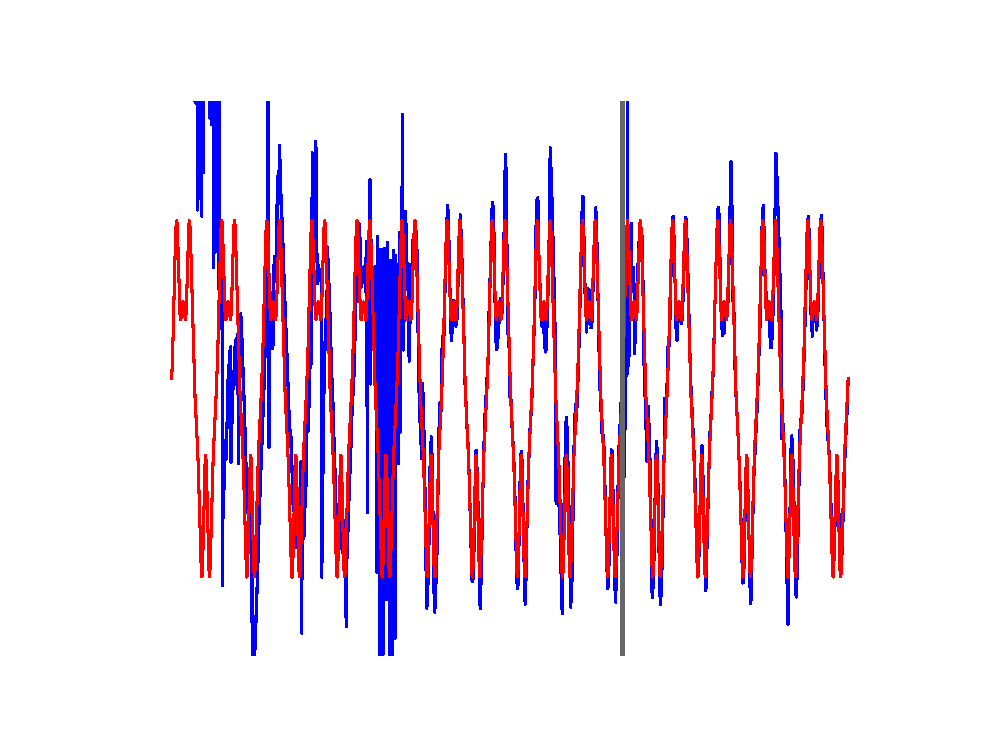
\includegraphics[trim=2cm 1cm 2cm 1cm, clip=true,height=0.1\linewidth,width=.45\linewidth]{Figures/Fig_T6/ImprovP/ST_T2_Seg7_Var_CoordinateY.eps}    
            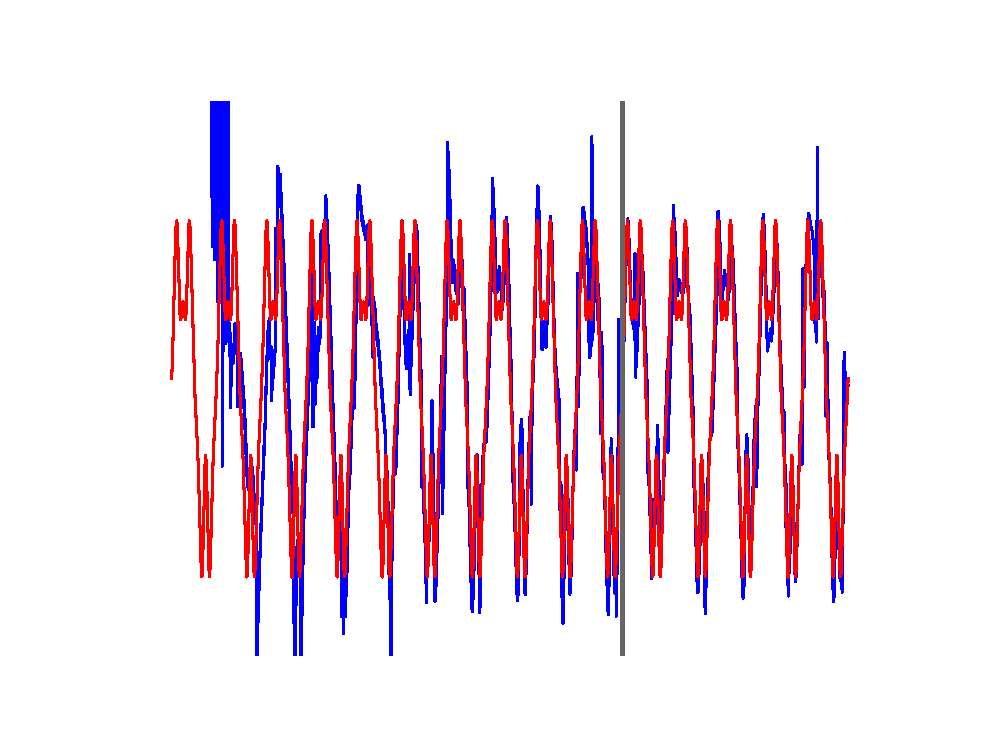
\includegraphics[trim=2cm 1cm 2cm 1cm, clip=true,height=0.1\linewidth,width=.45\linewidth]{Figures/Fig_T6/ImprovP/ST_T2_Seg8_Var_CoordinateY.eps} 

            \hspace{-1em}
            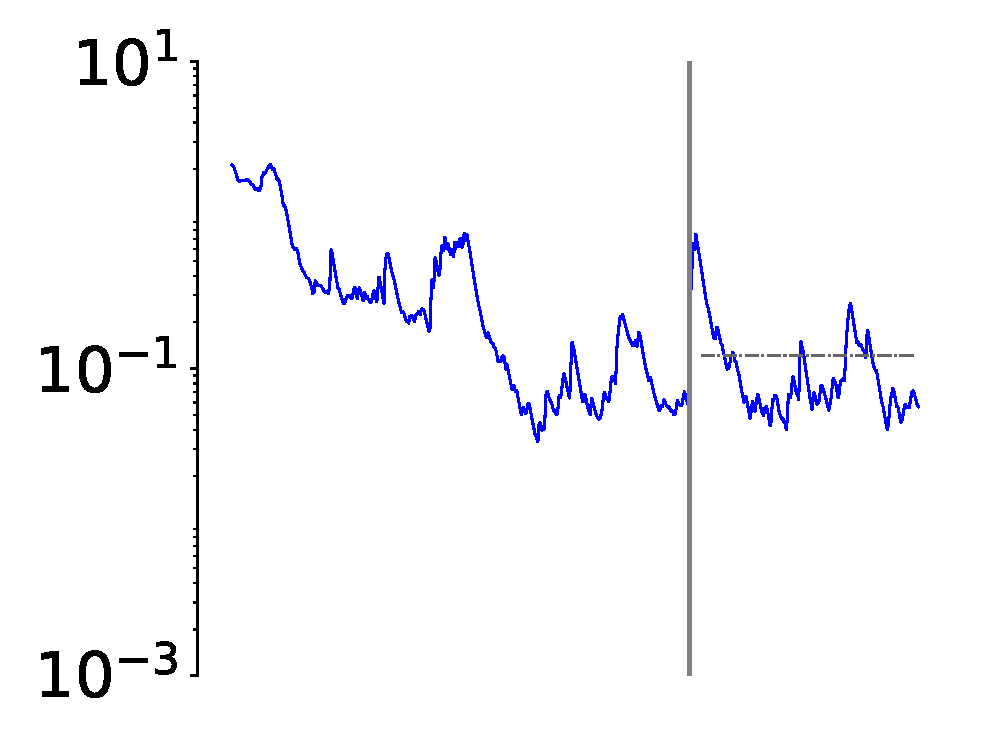
\includegraphics[height=0.15\linewidth,width=.45\linewidth]{Figures/Fig_T6/ImprovP/ST_T2_Seg7_Var_MSE.eps}
            \hspace{0em}
            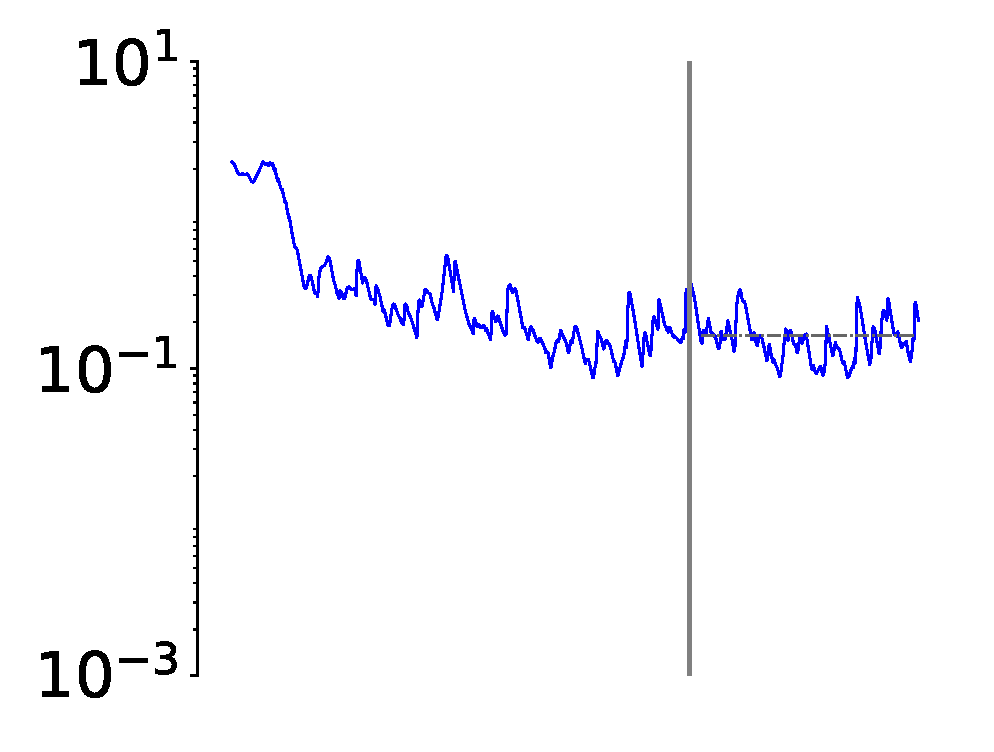
\includegraphics[height=0.15\linewidth,width=.45\linewidth]{Figures/Fig_T6/ImprovP/ST_T2_Seg8_Var_MSE.eps}
            
            
        \end{subfigure}
        
        \textbf{\rotatebox[origin=c]{90}{\hspace{-7.5em} MSE \hspace{2.5em} y(t) \hspace{1.5em} x(t)}}
        \begin{subfigure}{\textwidth}
            \centering
    
            \textbf{9 segments}\hspace{12em}\textbf{10 segments}
            
            
            
            
\includegraphics[trim=5cm 4cm 5cm 4cm, clip=true,height=0.15\linewidth]{Figures/Fig_T6/ImprovP/ST_T2_Seg9_Var_Trajectory.eps}
            \hspace{9em}
            \includegraphics[trim=5cm 4cm 5cm 4cm, clip=true,height=0.15\linewidth]{Figures/Fig_T6/ImprovP/ST_T2_Seg10_Var_Trajectory.eps}
            %trim=1cm 0cm 0cm 0cm, clip=true,
            
            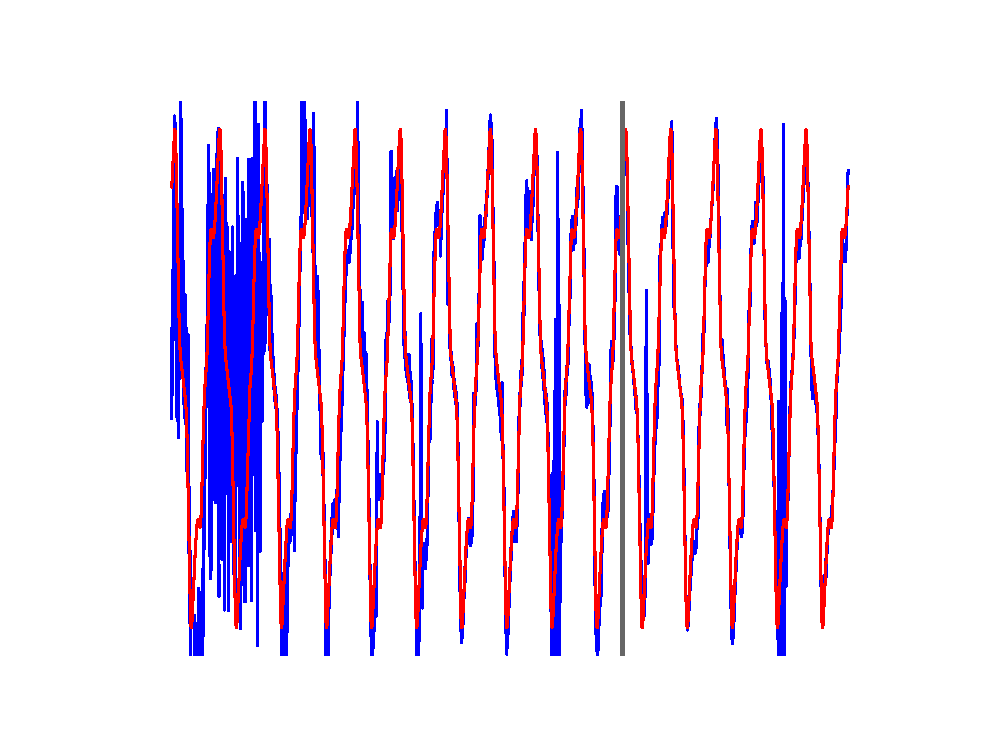
\includegraphics[trim=2cm 1cm 2cm 1cm, clip=true,height=0.1\linewidth,width=.45\linewidth]{Figures/Fig_T6/ImprovP/ST_T2_Seg9_Var_CoordinateX.eps} 
            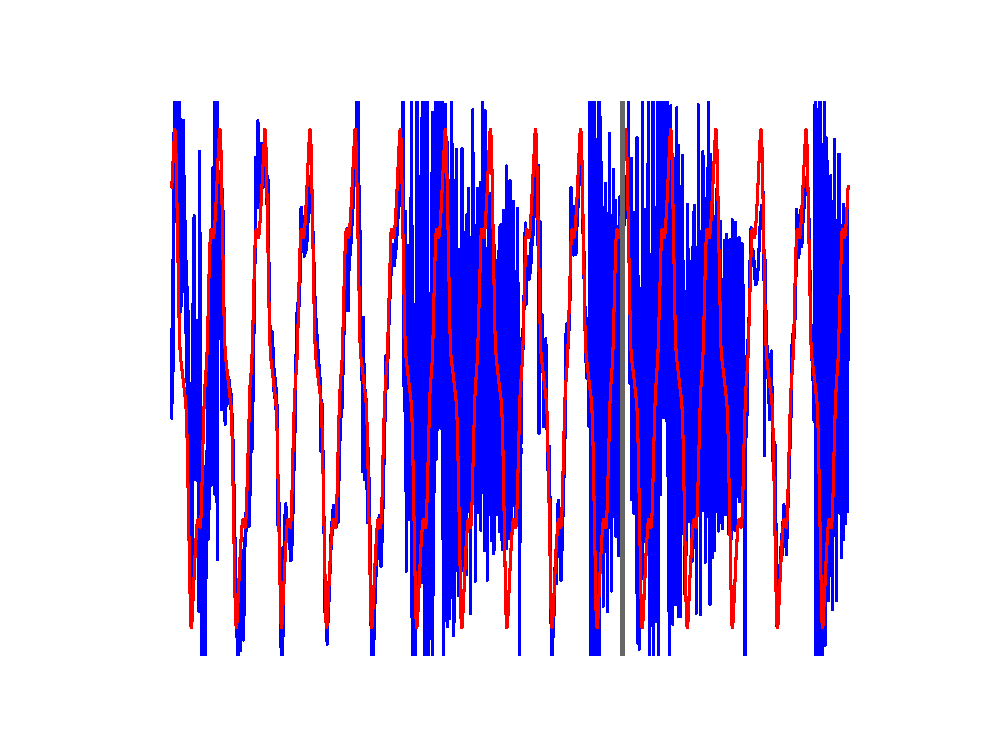
\includegraphics[trim=2cm 1cm 2cm 1cm, clip=true,height=0.1\linewidth,width=.45\linewidth]{Figures/Fig_T6/ImprovP/ST_T2_Seg10_Var_CoordinateX.eps}       

            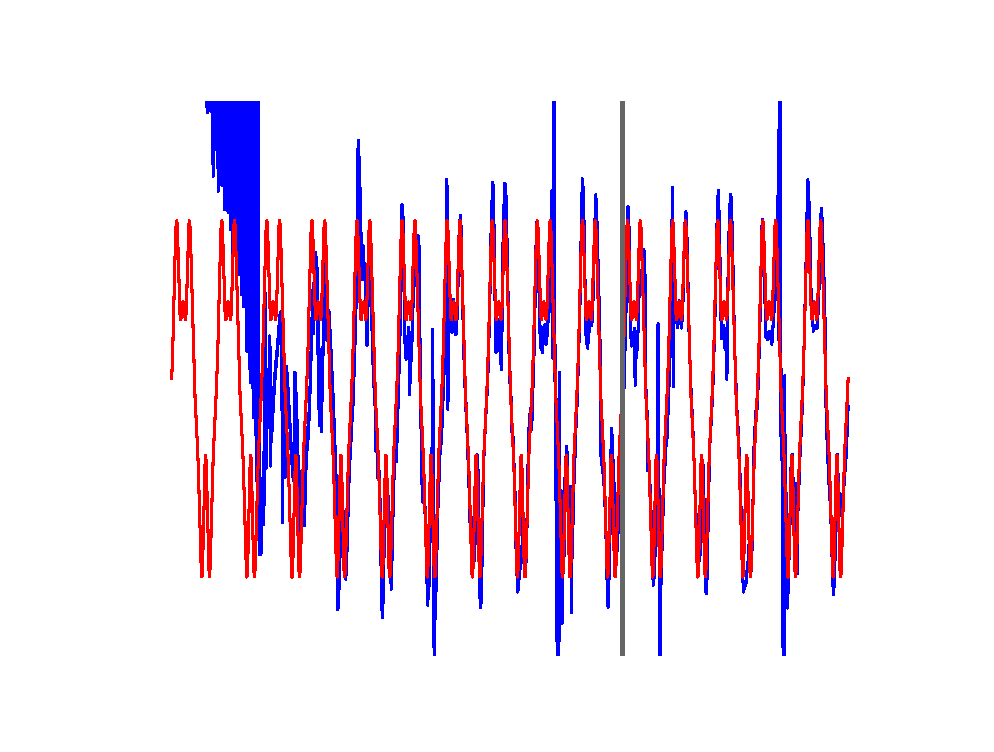
\includegraphics[trim=2cm 1cm 2cm 1cm, clip=true,height=0.1\linewidth,width=.45\linewidth]{Figures/Fig_T6/ImprovP/ST_T2_Seg9_Var_CoordinateY.eps}    
            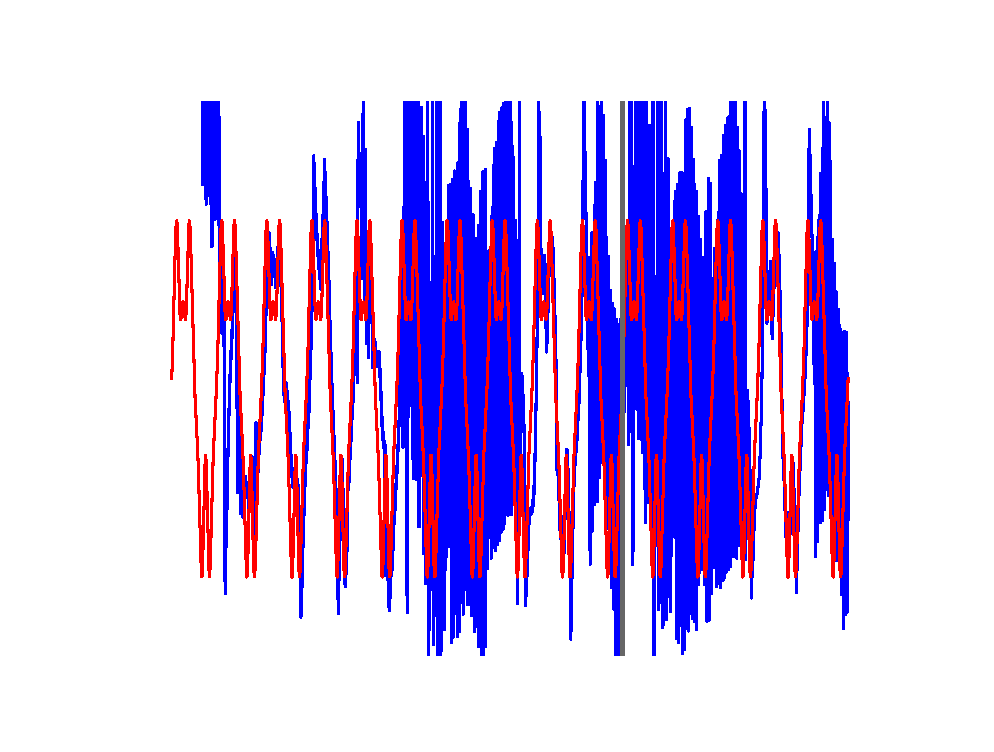
\includegraphics[trim=2cm 1cm 2cm 1cm, clip=true,height=0.1\linewidth,width=.45\linewidth]{Figures/Fig_T6/ImprovP/ST_T2_Seg10_Var_CoordinateY.eps} 

            \hspace{-1em}
            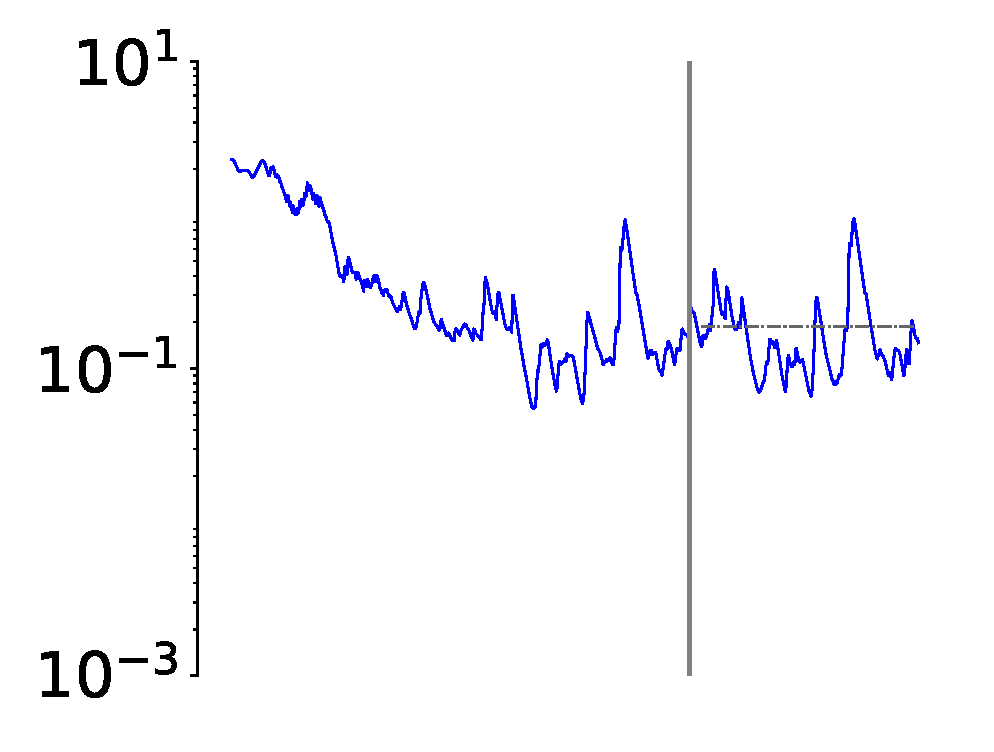
\includegraphics[height=0.15\linewidth,width=.45\linewidth]{Figures/Fig_T6/ImprovP/ST_T2_Seg9_Var_MSE.eps}
            \hspace{0em}
            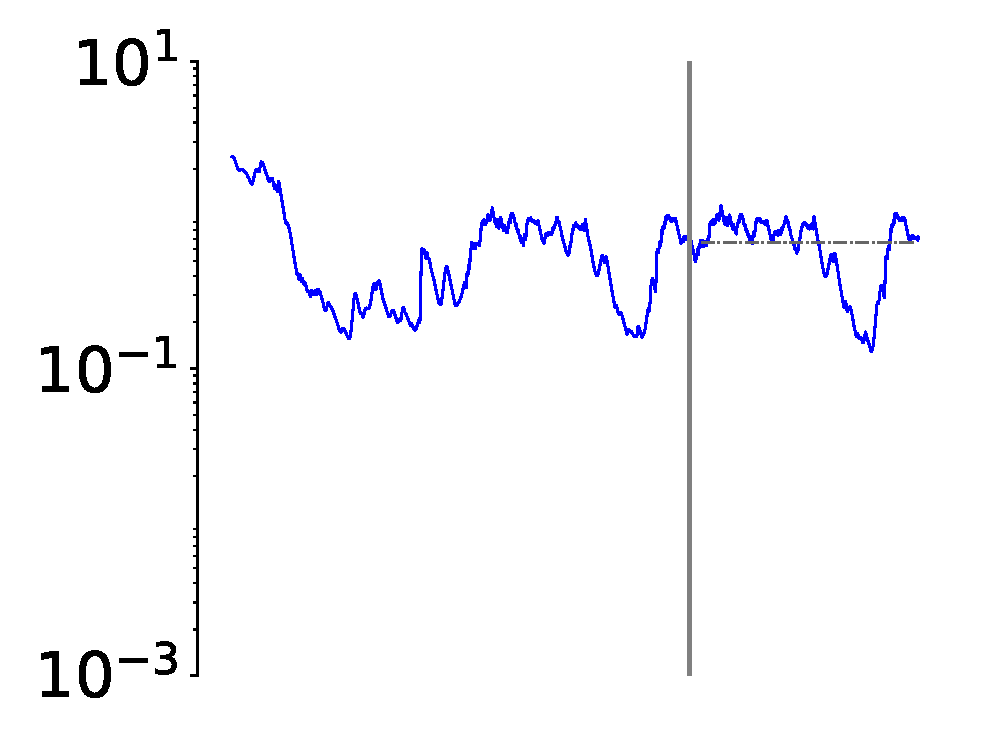
\includegraphics[height=0.15\linewidth,width=.45\linewidth]{Figures/Fig_T6/ImprovP/ST_T2_Seg10_Var_MSE.eps}
            
        \end{subfigure}
    \caption{Scalability of the performance of the modified Python re-implementation using the SUPERTREX algorithm on Task 2. The lengths of the arm segments are 1.8, 1.2 and 0.6 for the first three segments (akin to Task 3) and 0.1 for each additional segment. Here, the simulations for Task 2 with 5 to 50 segments are shown, all using the default seed 5489 for the random number generator. (Continued on next page.)}
    \label{Fig:Scalability_Task2}

\end{figure}
    
    
    
    
\begin{figure}
\ContinuedFloat
        \textbf{\rotatebox[origin=c]{90}{\hspace{-7.5em} MSE \hspace{2.5em} y(t) \hspace{1.5em} x(t)}}
        \begin{subfigure}{\textwidth}
            \centering
    
            \textbf{20 segments}\hspace{12em}\textbf{30 segments}
            
            
            
            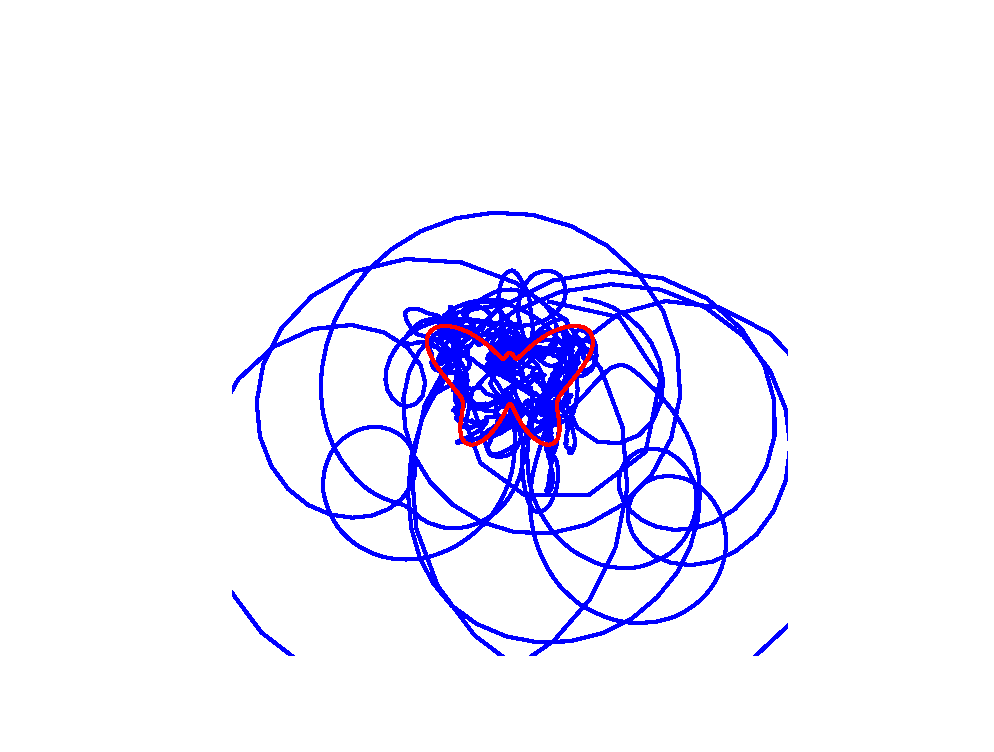
\includegraphics[trim=5cm 4cm 5cm 4cm, clip=true,height=0.15\linewidth]{Figures/Fig_T6/ImprovP/ST_T2_Seg20_Var_Trajectory.eps}
            \hspace{9em}
            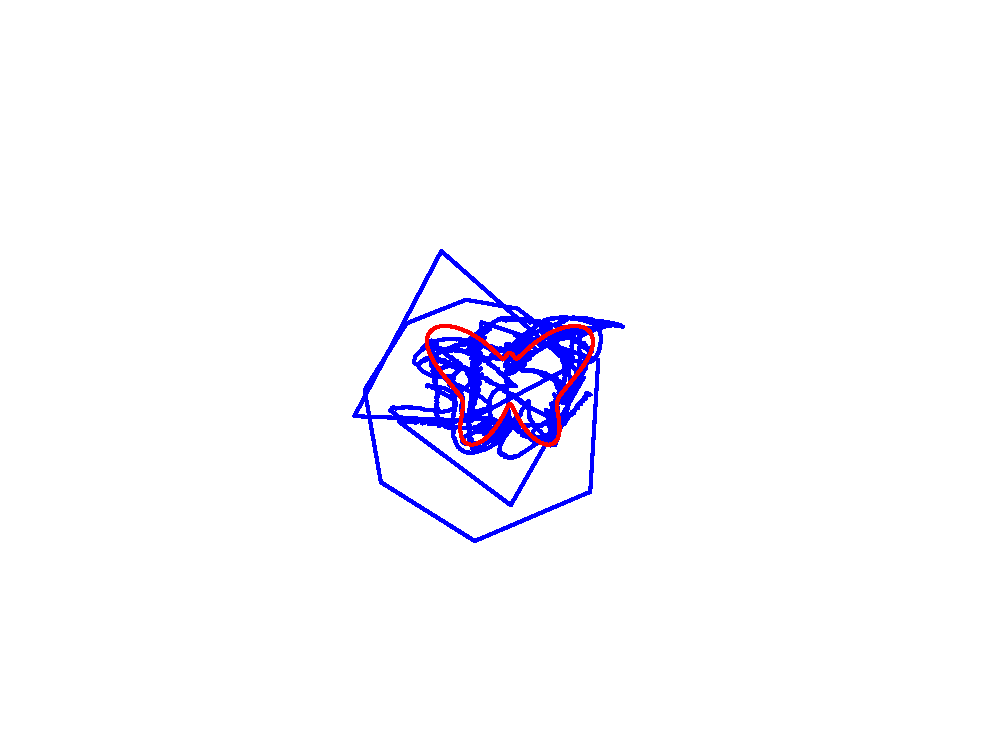
\includegraphics[trim=5cm 4cm 5cm 4cm, clip=true,height=0.15\linewidth]{Figures/Fig_T6/ImprovP/ST_T2_Seg30_Var_Trajectory.eps}
            %trim=1cm 0cm 0cm 0cm, clip=true,
            
            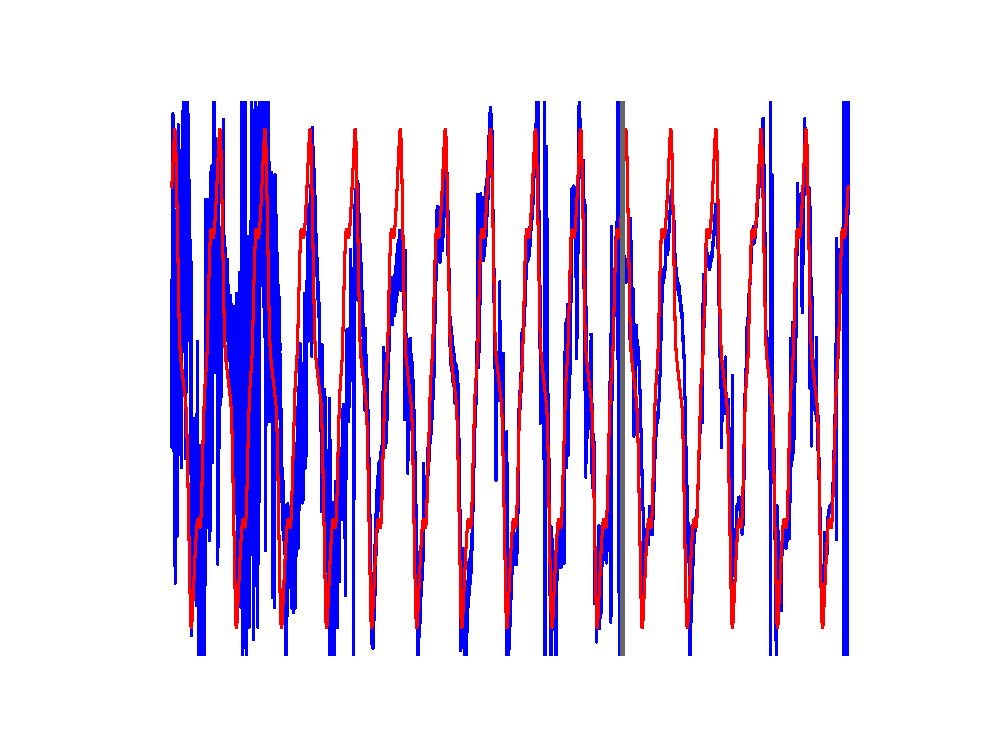
\includegraphics[trim=2cm 1cm 2cm 1cm, clip=true,height=0.1\linewidth,width=.45\linewidth]{Figures/Fig_T6/ImprovP/ST_T2_Seg20_Var_CoordinateX.eps} 
            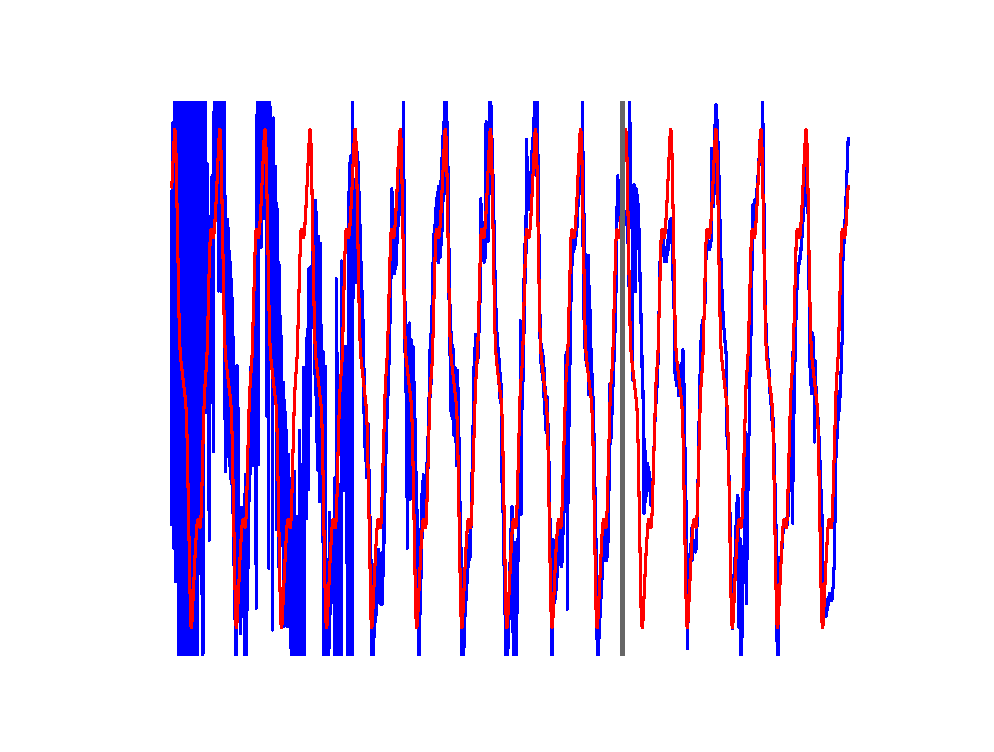
\includegraphics[trim=2cm 1cm 2cm 1cm, clip=true,height=0.1\linewidth,width=.45\linewidth]{Figures/Fig_T6/ImprovP/ST_T2_Seg30_Var_CoordinateX.eps}       

            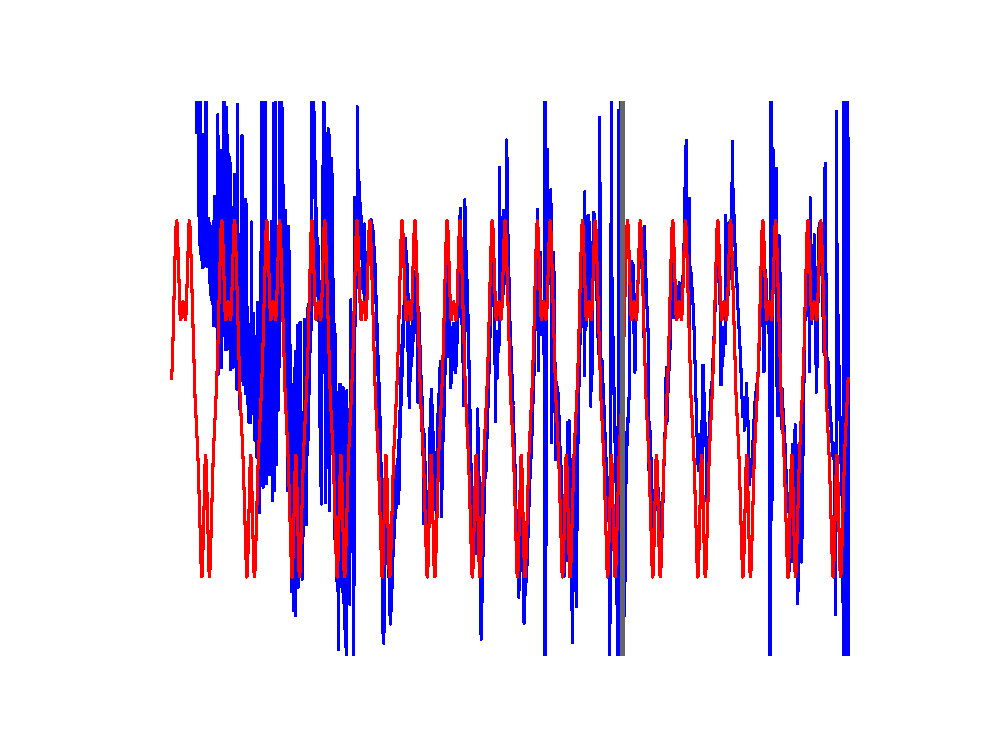
\includegraphics[trim=2cm 1cm 2cm 1cm, clip=true,height=0.1\linewidth,width=.45\linewidth]{Figures/Fig_T6/ImprovP/ST_T2_Seg20_Var_CoordinateY.eps}    
            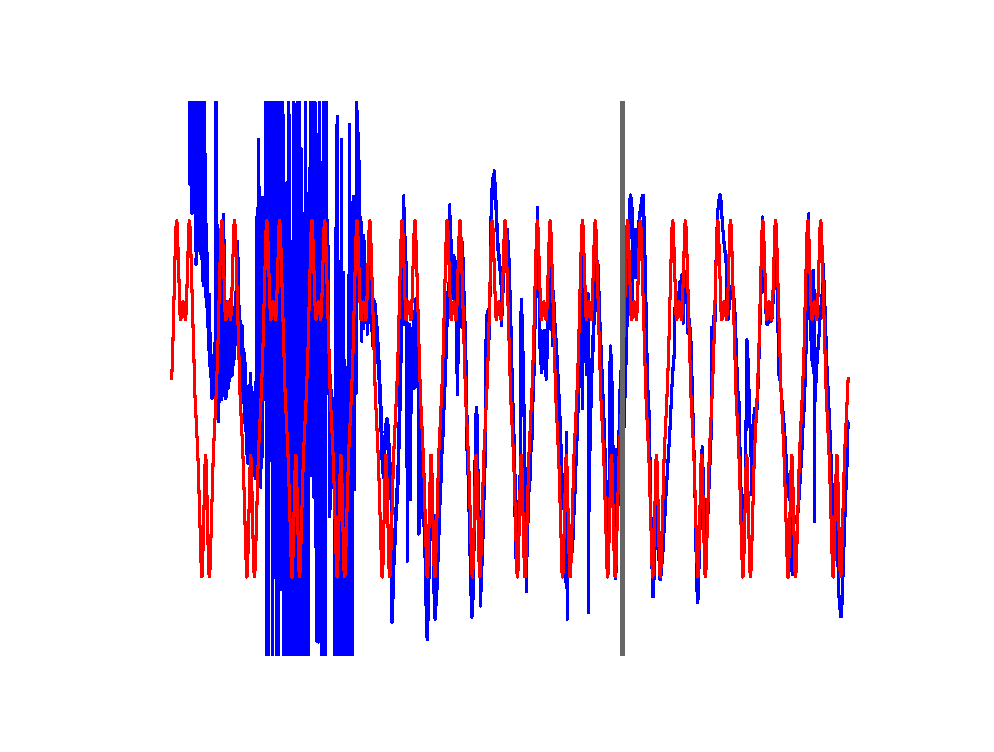
\includegraphics[trim=2cm 1cm 2cm 1cm, clip=true,height=0.1\linewidth,width=.45\linewidth]{Figures/Fig_T6/ImprovP/ST_T2_Seg30_Var_CoordinateY.eps} 

            \hspace{-1em}
            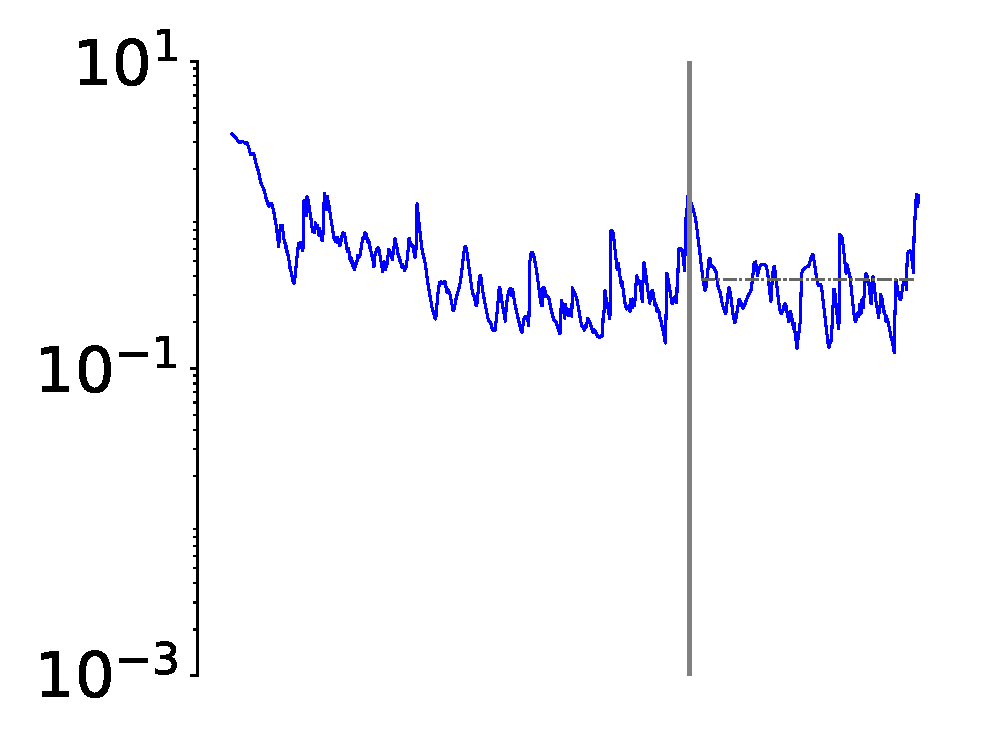
\includegraphics[height=0.15\linewidth,width=.45\linewidth]{Figures/Fig_T6/ImprovP/ST_T2_Seg20_Var_MSE.eps}
            \hspace{0em}
            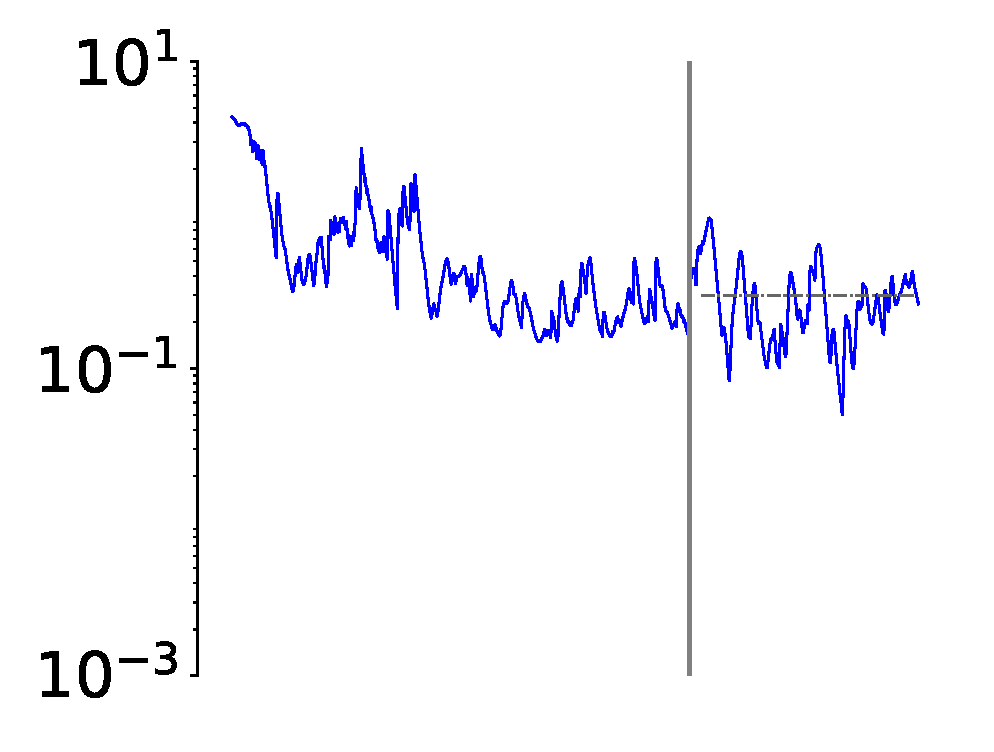
\includegraphics[height=0.15\linewidth,width=.45\linewidth]{Figures/Fig_T6/ImprovP/ST_T2_Seg30_Var_MSE.eps}
            
        \end{subfigure}
        
        \textbf{\rotatebox[origin=c]{90}{\hspace{-7.5em} MSE \hspace{2.5em} y(t) \hspace{1.5em} x(t)}}
        \begin{subfigure}{\textwidth}
            \centering
    
            \textbf{40 segments}\hspace{12em}\textbf{50 segments}
            
            
            
            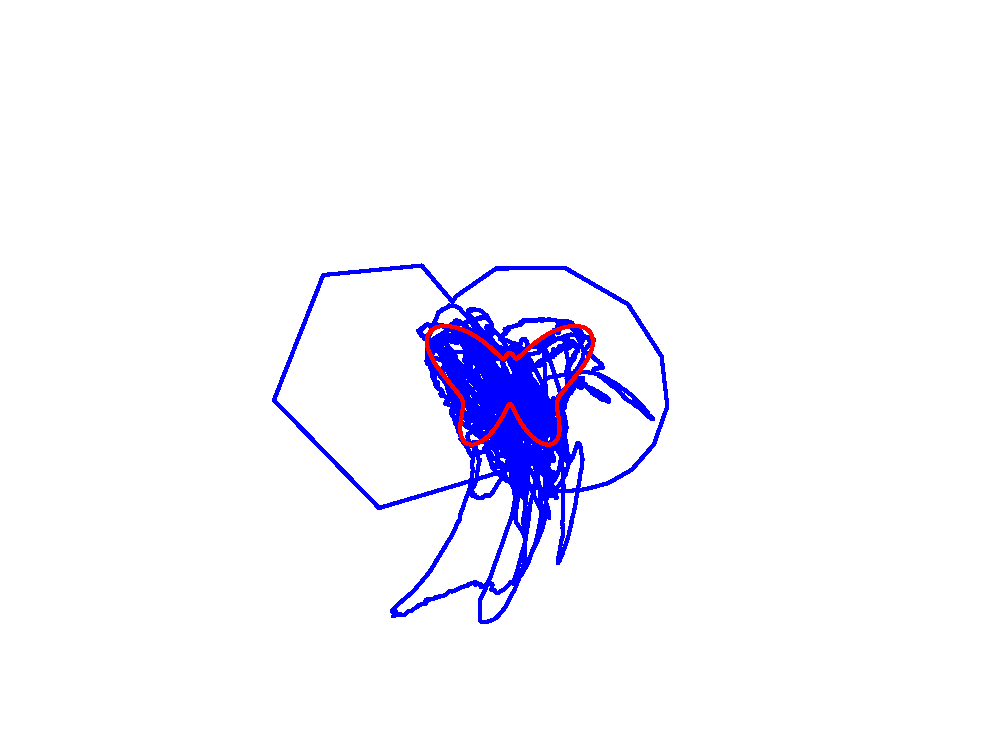
\includegraphics[trim=5cm 4cm 5cm 4cm, clip=true,height=0.15\linewidth]{Figures/Fig_T6/ImprovP/ST_T2_Seg40_Var_Trajectory.eps}
            \hspace{9em}
            \includegraphics[trim=5cm 4cm 5cm 4cm, clip=true,height=0.15\linewidth]{Figures/Fig_T6/ImprovP/ST_T2_Seg50_Var_Trajectory.eps}
            %trim=1cm 0cm 0cm 0cm, clip=true,
            
            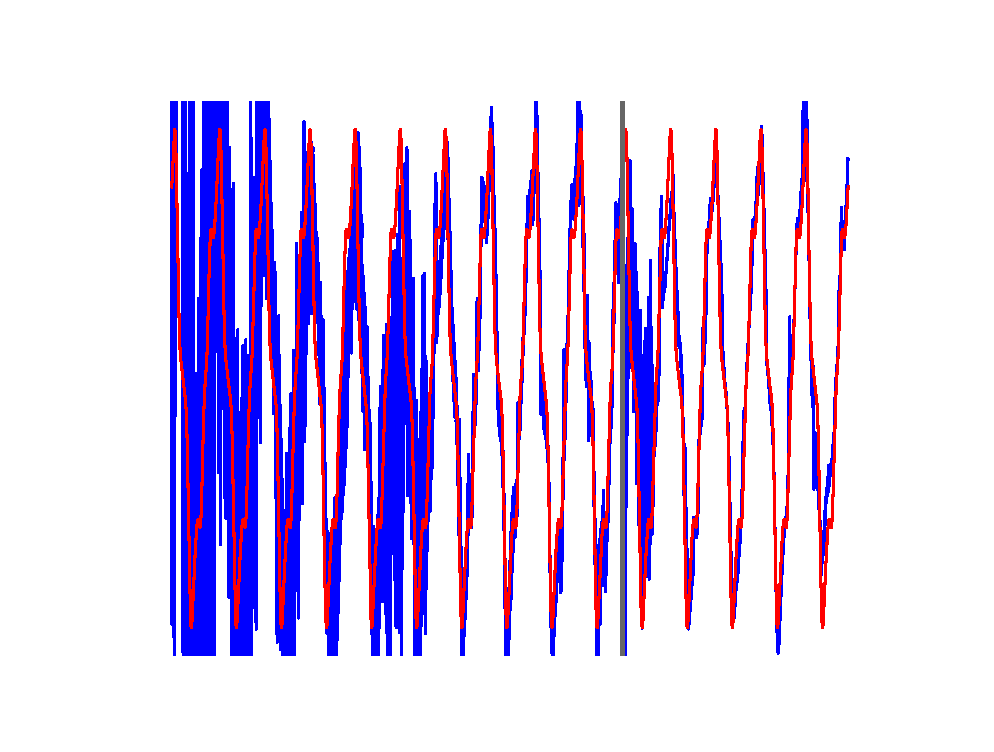
\includegraphics[trim=2cm 1cm 2cm 1cm, clip=true,height=0.1\linewidth,width=.45\linewidth]{Figures/Fig_T6/ImprovP/ST_T2_Seg40_Var_CoordinateX.eps} 
            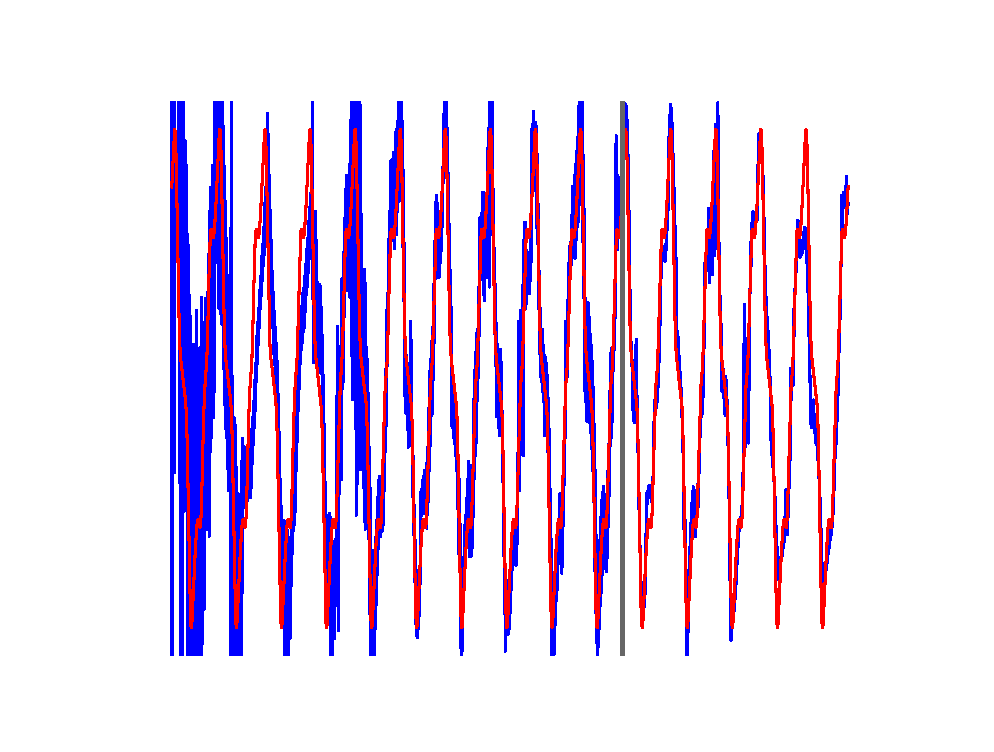
\includegraphics[trim=2cm 1cm 2cm 1cm, clip=true,height=0.1\linewidth,width=.45\linewidth]{Figures/Fig_T6/ImprovP/ST_T2_Seg50_Var_CoordinateX.eps}       

            \includegraphics[trim=2cm 1cm 2cm 1cm, clip=true,height=0.1\linewidth,width=.45\linewidth]{Figures/Fig_T6/ImprovP/ST_T2_Seg40_Var_CoordinateY.eps}    
            \includegraphics[trim=2cm 1cm 2cm 1cm, clip=true,height=0.1\linewidth,width=.45\linewidth]{Figures/Fig_T6/ImprovP/ST_T2_Seg50_Var_CoordinateY.eps} 

            \hspace{-1em}
            \includegraphics[height=0.15\linewidth,width=.45\linewidth]{Figures/Fig_T6/ImprovP/ST_T2_Seg40_Var_MSE.eps}
            \hspace{0em}
            \includegraphics[height=0.15\linewidth,width=.45\linewidth]{Figures/Fig_T6/ImprovP/ST_T2_Seg50_Var_MSE.eps}
            
        \end{subfigure}
        
        
        
    
        
        \includegraphics[trim=2cm 6cm 2cm 6cm, clip=true,height=0.05\linewidth,width=.4\linewidth]{Figures/Fig_T1/Python/ST_T1_Scale.eps}
        \includegraphics[trim=2cm 4cm 2cm 6cm, clip=true,height=0.05\linewidth,width=.45\linewidth]{Figures/Fig_T1/Python/ST_T1_Scale.eps}
    


    \caption{(Continued from previous page.) Scalability of the performance of the modified Python re-implementation using the SUPERTREX algorithm on Task 2. The lengths of the arm segments are 1.8, 1.2 and 0.6 for the first three segments (akin to Task 3) and 0.1 for each additional segment. Here, the simulations for Task 2 with 5 to 50 segments are shown, all using the default seed 5489 for the random number generator. In each subfigure, the top panel shows the produced trajectory, the middle panels show the evolution of the x and y coordinates of the end-effector of the arm (blue) throughout the training and test phase, along with the target coordinates (red). The grey vertical line marks the separation of the training and testing phase. The bottom panel shows the progression of the distance from target metric (blue) over the simulation, using the log scale for the y axis. The horizontal grey line, in the test phase, indicates the deviation metric.}
    \label{Fig:Scalability_Task2_cont}

\end{figure}

